% !TEX root = handbook-physics.tex
% !TEX TS-program = pdflatex
% !TEX encoding = UTF-8 Unicode






\chapter{Electromagnetic Waves}
\label{ch-31}
\zhtitle{电磁波}

\section{Properties of Electromagnetic Waves}
\label{sec-31.1} 
\zhtitle{电磁波的性质}


\subsection{}\label{31.1.1} \redem{Electromagnetic waves} are disturbances of an electromagnetic field (i.e. a variable electromagnetic field) that propagate through space. The statement of the existence of electromagnetic waves follows directly from Maxwell's equations \ssect{27.4.3}. For an electromagnetic field, distant from the free electric charges \ssect{18.3.1} and macroscopic currents \ssect{26.4.1} that
it was set up by, these equations are of the form:\sidenote{All equations in Chapter~\ref{ch-31} are written in SI units.}
\zhpar{\redem{电磁波}是在空间中传播的电磁场（即变化的电磁场）的扰动。电磁波存在的结论可直接由麦克斯韦方程组\ssect{27.4.3}得出。对于远离产生该场的自由电荷\ssect{18.3.1}和宏观电流\ssect{26.4.1}的电磁场，这些方程的形式为：}
\zhpar{注：本章所有公式均采用国际单位制。}
\[
\begin{alignedat}{2}
\curl \vb{E} & = - \pdv{\vb{B}}{t}, & \quad \curl \vb{H} & = \pdv{\vb{D}}{t}, \\
\div \vb{D} & = 0,                  & \quad \div \vb{B} & = 0.
\end{alignedat}
\]
 \subsection{}\label{31.1.2} If the medium is a uniform and isotropic dielectric \ssect{30.1.6}, having no ferroelectric \ssect{18.4.1} or ferromagnetic \ssect{26.5.1} properties, then $\vb{D} = \varepsilon_{r}\varepsilon_{0}\vb{E}$ and $\vb{B} = \mu_{r}\mu_{0}\vb{H}$, where
$\varepsilon_{r}$ and $\mu_{r}$ are constant scalar quantities independent both of the coordinates and of time. Here Maxwell's equations \ssect{31.1.1} can be rewritten in the form
\zhpar{若介质为均匀各向同性的电介质，且不具有铁电性\ssect{18.4.1}或铁磁性\ssect{26.5.1}，则 $\vb{D} = \varepsilon_{r}\varepsilon_{0}\vb{E}$，$\vb{B} = \mu_{r}\mu_{0}\vb{H}$，其中 $\varepsilon_{r}$ 与 $\mu_{r}$ 为与坐标和时间均无关的常量。此时，麦克斯韦方程组\ssect{31.1.1}可改写为下列形式：}
\[
\begin{alignedat}{2}
\curl \vb{E} & = - \mu_{r} \mu_{0} \pdv{\vb{H}}{t}, & \quad \curl \vb{H} & = \varepsilon_{r} \varepsilon_{0} \pdv{\vb{E}}{t}, \\
\div \vb{E} & = 0,                                 & \quad \div \vb{H} & = 0.
\end{alignedat}
\]
or in projections on the axes of Cartesian coordinates:
\zhpar{或写成笛卡儿直角坐标轴上各分量的形式：}
\[
\begin{alignedat}{2}
\pdv{E_{z}}{y}& - \pdv{E_{y}}{z}  = - \mu_{r} \mu_{0} \pdv{H_{x}}{t}, 
& \quad \pdv{H_{z}}{y} & - \pdv{H_{y}}{z}  = \varepsilon_{r} \varepsilon_{0} \pdv{E_{x}}{t}, \\
\pdv{E_{x}}{z} & - \pdv{E_{z}}{x} = - \mu_{r} \mu_{0} \pdv{H_{y}}{t}, 
& \quad \pdv{H_{x}}{z} & - \pdv{H_{z}}{x} = \varepsilon_{r} \varepsilon_{0} \pdv{E_{y}}{t}, \\
\pdv{E_{y}}{x} & - \pdv{E_{x}}{y} = - \mu_{r} \mu_{0} \pdv{H_{z}}{t}, 
& \quad \pdv{H_{y}}{x} & - \pdv{H_{x}}{y} = \varepsilon_{r} \varepsilon_{0} \pdv{E_{z}}{t},\\
\pdv{E_{x}}{x} & + \pdv{E_{y}}{y} + \pdv{E_{z}}{z} = 0, & \quad \pdv{H_{x}}{x} & + \pdv{H_{y}}{y} + \pdv{H_{z}}{z}  = 0. 
\end{alignedat}
\]

\subsection{}\label{31.1.3} It follows from Maxwell's equations \ssect{31.1.2} that the
strength vectors $\vb{E}$ and $\vb{H}$ of a variable electromagnetic field and their projections onto the axes of Cartesian coordinates comply in a uniform, isotropic, nonconducting medium, with the wave equation \ssect{30.2.9}:
\zhpar{由麦克斯韦方程组\ssect{31.1.2}可知，在均匀、各向同性、不导电的介质中，变化电磁场的强度矢量 $\vb{E}$ 与 $\vb{H}$ 及其在笛卡儿直角坐标轴上的投影，都满足波动方程\ssect{30.2.9}：}
\[
\begin{alignedat}{2}
\Delta \vb{E} - \varepsilon_{r} \varepsilon_{0}\mu_{r} \mu_{0} \pdv[2]{\vb{E}}{t} & = 0, &  \quad \Delta \vb{H} - \varepsilon_{r} \varepsilon_{0}\mu_{r} \mu_{0} \pdv[2]{\vb{H}}{t} & = 0,\\
\Delta E_{x} - \varepsilon_{r} \varepsilon_{0}\mu_{r} \mu_{0} \pdv[2]{E_{x}}{t} & = 0, & \quad  \Delta E_{y} - \varepsilon_{r} \varepsilon_{0}\mu_{r} \mu_{0} \pdv[2]{E_{y}}{t} & = 0,\\
\Delta E_{z} - \varepsilon_{r} \varepsilon_{0}\mu_{r} \mu_{0} \pdv[2]{E_{z}}{t} & = 0, & \quad \\
\Delta H_{x} - \varepsilon_{r} \varepsilon_{0}\mu_{r} \mu_{0} \pdv[2]{H_{x}}{t} & = 0, & \quad  \Delta H_{y} - \varepsilon_{r} \varepsilon_{0}\mu_{r} \mu_{0} \pdv[2]{H_{y}}{t} & = 0,\\
\Delta H_{z} - \varepsilon_{r} \varepsilon_{0}\mu_{r} \mu_{0} \pdv[2]{H_{z}}{t} & = 0.
\end{alignedat}
\]
Thus a variable electromagnetic field really propagates in space
in the form of waves with the phase velocity
\zhpar{因此，变化的电磁场确实以波的形式在空间中传播，其相速度为}
\begin{equation*}%
v = \frac{c}{\sqrt{\varepsilon_{r} \mu_{r}}}, \,\, \text{where} \,\, c =\frac{1}{\sqrt{\varepsilon_{0} \mu_{0}}} = \SI{3d8}{\meter\per\second}.
\end{equation*}
In vacuum $\varepsilon_{r} = \mu_{r} = 1$. Hence, $c$ is the \redem{velocity of electromagnetic waves} in vacuum (in free space).
\zhpar{在真空中 $\varepsilon_{r} = \mu_{r} = 1$，因此 $c$ 即为真空（自由空间）中\redem{电磁波的速度}。}

\subsection{}\label{31.1.4} Electromagnetic waves are \redem{transverse} waves: vectors $\vb{E}$ and $\vb{H}$ of the field lie in a plane perpendicular to the direction of wave propagation, i.e. to the wave velocity vector $\vb{v}$ at the point being considered in the field. This can he most readily demonstrated by the example of a plane wave, propagating along the positive direction of axis $OX$ \ssect{30.2.4}:
\zhpar{电磁波是\redem{横波}：矢量 $\vb{E}$ 与 $\vb{H}$ 位于垂直于传播方向（即场中该点处的波速矢量 $\vb{v}$）的平面内。最容易通过沿 $OX$ 轴正方向传播的平面波来说明这一点\ssect{30.2.4}：}
\begin{equation*}%
\vb{E} = f\,\left(t - \frac{x}{v} \right) \qand \vb{H} = \varphi\,\left(t - \frac{x}{v} \right).
\end{equation*}
Vector $\vb{E}$ and $\vb{H}$ and their projections on the coordinate axes are independent of $y$ and $z$:
\zhpar{矢量 $\vb{E}$ 与 $\vb{H}$ 及其在坐标轴上的投影均与 $y$ 和 $z$ 无关：}
\begin{align*}%
\pdv{E_{x}}{y} & = \pdv{E_{x}}{z}= \pdv{E_{y}}{y} =\pdv{E_{y}}{z}= \pdv{E_{z}}{y}= \pdv{E_{z}}{z} =0 \qand \\
\pdv{H_{x}}{y} & = \pdv{H_{x}}{z}= \pdv{H_{y}}{y} =\pdv{H_{y}}{z}= \pdv{H_{z}}{y}= \pdv{H_{z}}{z}
\end{align*}
It follows from Maxwell's equations \ssect{31.1.2} that for the field of a plane wave,
\zhpar{由麦克斯韦方程组\ssect{31.1.2}可知，对于平面波的场，有}
\begin{equation*}%
\pdv{E_{x}}{x} = \pdv{E_{x}}{t} = 0 \qand \pdv{H_{x}}{x} = \pdv{H_{x}}{t} = 0,
\end{equation*}
i.e. $E_{x}$ and $H_{x}$ are independent of both coordinates and time.
\zhpar{即 $E_{x}$ 与 $H_{x}$ 与坐标和时间均无关。}

Hence, for a \redem{variable} field of a plane  wave $E_{x} = H_{x} = 0$, and the vectors $\vb{E}$ and $\vb{H}$ are perpendicular to the direction of wave propagation:
\zhpar{因此，对于平面波的\redem{变化}场，$E_{x} = H_{x} = 0$，矢量 $\vb{E}$ 与 $\vb{H}$ 均垂直于波的传播方向：}
\begin{equation*}%
\vb{E} = E_{y}\vu{j} + E_{z}\vu{k} \qand \vb{H} = H_{y}\vu{j} + H_{z}\vu{k} 
\end{equation*}
where $\vu{j}$ and $\vu{k}$ are unit vectors of the
coordinate axes.
\zhpar{式中 $\vu{j}$ 与 $\vu{k}$ 为坐标轴方向的单位矢量。}

\begin{marginfigure}%[-1.5cm]
\centering
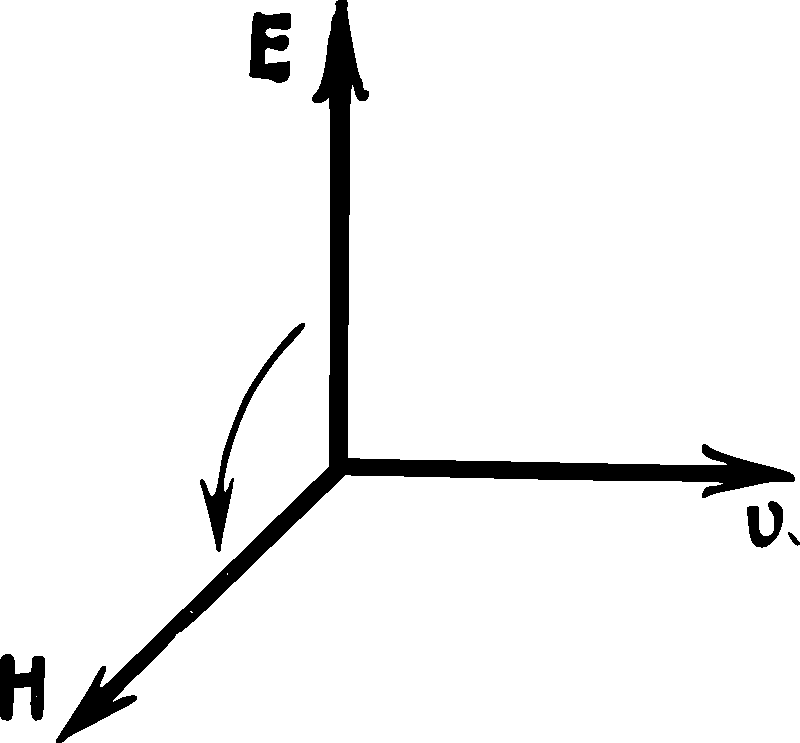
\includegraphics[width=0.7\textwidth]{figs/ch-31/fig-31-01.pdf}
\sidecaption{Mutually perpendicular vectors $\vb{E}$ and $\vb{H}$ of the field of an electromagnetic wave.\zhcap{电磁波场中相互垂直的矢量 $\vb{E}$ 与 $\vb{H}$。}\label{fig-31-01}}
\end{marginfigure}

\subsection{}\label{31.1.5} Vectors $\vb{E}$ and $\vb{H}$ of the field of an electromagnetic wave are mutually perpendicular, so that $\vb{v}$, $\vb{E}$ and $\vb{H}$ form a right-hand set of three vectors (\figr{fig-31-01}).
\zhpar{电磁波场中的矢量 $\vb{E}$ 与 $\vb{H}$ 相互垂直，因此 $\vb{v}$、$\vb{E}$ 与 $\vb{H}$ 构成右手系的三个矢量（见\figr{fig-31-01}）。}

As a matter of fact, for the field of a plane wave \ssect{31.1.4},
\zhpar{事实上，对于平面波的场\ssect{31.1.4}，有}
\begin{align*}%
E_{y} & = f_{1}\,\left(t - \frac{x}{v} \right) \qand E_{z} = f_{2}\,\left(f - \frac{x}{v} \right),\\
H_{y} & = \varphi_{1}\,\left(t - \frac{x}{v} \right) \qand E_{z} = f_{2}\,\left(f - \frac{x}{v} \right),\\
\end{align*}
It follows from Maxwell's equations \ssect{31.1.2} that
\zhpar{由麦克斯韦方程组\ssect{31.1.2}可得}
\begin{align*}%
\sqrt{\varepsilon_{r} \varepsilon_{0}}\pdv{E_{y}}{\xi} & = \sqrt{\mu_{r} \mu_{0}} \pdv{H_{z}}{\xi} \qand \\
\sqrt{\varepsilon_{r} \varepsilon_{0}}\pdv{E_{z}}{\xi} & = - \sqrt{\mu_{r} \mu_{0}} \pdv{H_{y}}{\xi} \qand \\
\end{align*}
where $\xi = t - x/v$. Therefore, for a variable field of a plane
wave
\zhpar{式中 $\xi = t - x/v$。因此，对于平面波的变化场，有}
\begin{equation*}%
H_{y} = - \sqrt{\frac{\varepsilon_{r} \varepsilon_{0}}{\mu_{r} \mu_{0}}} E_{z}, \quad H_{z} = - \sqrt{\frac{\varepsilon_{r} \varepsilon_{0}}{\mu_{r} \mu_{0}}} E_{y}, \qand (\vb{E}\vb{H}) = 0.
\end{equation*}
The mutually perpendicular vectors $\vb{E}$ and $\vb{H}$ oscillate in phase: they become zero simultaneously and reach their maximum
values simultaneously. The relation between their magnitudes is
\zhpar{相互垂直的矢量 $\vb{E}$ 与 $\vb{H}$ 同相振动：二者同时为零，同时达到最大值。二者大小之间的关系为}
\begin{equation*}%
\sqrt{\varepsilon_{r} \varepsilon_{0}}E= \sqrt{\mu_{r} \mu_{0}} H,
\end{equation*}
which is valid for any travelling electromagnetic wave \ssect{30.2.1} regardless of the shape of its wavefronts \ssect{30.2.3}.
\zhpar{该关系对任何行波形式的电磁波都成立\ssect{30.2.1}，与其波面的形状无关\ssect{30.2.3}。}

\subsection{}\label{31.1.6} A \redem{monochromatic wave} is an electromagnetic wave of a single definite frequence $\nu$, i.e. an electromagnetic sine wave. At each point of the electromagnetic field of a monochromatic wave, the projections of vectors $\vb{E}$ and $\vb{H}$ on the coordinate axes of an inertial frame of reference have harmonic oscillations \ssect{28.1.3} of the same frequency, equal to the wave frequency $\nu$.
\zhpar{\redem{单色波}是指具有单一确定频率 $\nu$ 的电磁波，即电磁正弦波。在单色波电磁场的每一点，矢量 $\vb{E}$ 与 $\vb{H}$ 在惯性参考系坐标轴上的投影都做频率相同（等于波的频率 $\nu$）的简谐振动\ssect{28.1.3}。}

For example, in the case of a \redem{plane monochromatic wave}, propagating along the positive direction of axis $OX$,
\zhpar{例如，对于沿 $OX$ 轴正方向传播的\redem{平面单色波}，}
\begin{align*}%
E_{y} & = A_{1} \sin (\omega t - kx),\quad & H_{y} & = - \sqrt{\frac{\varepsilon_{r} \varepsilon_{0}}{\mu_{r} \mu_{0}}} E_{z},\\
E_{z} & = A_{1} \sin (\omega t - kx + \varphi),\quad  & H_{z} & = - \sqrt{\frac{\varepsilon_{r} \varepsilon_{0}}{\mu_{r} \mu_{0}}} E_{y},
\end{align*}
where $\omega = 2\pi \nu$ is the angular frequency of the wave, $k$ is the wavenumber \ssect{30.2.6}, $A_{1}$ and $A_{2}$ are the amplitudes of $E_{y}$ and $E_{z}$, and $\varphi$ is the phase difference between the oscillations of $E_{z}$ and $E_{y}$.
\zhpar{式中 $\omega = 2\pi \nu$ 为波的角频率，$k$ 为波数\ssect{30.2.6}，$A_{1}$ 与 $A_{2}$ 分别为 $E_{y}$ 与 $E_{z}$ 的振幅，$\varphi$ 为 $E_{z}$ 与 $E_{y}$ 振动之间的相位差。}

\begin{marginfigure}%[-1.5cm]
\centering
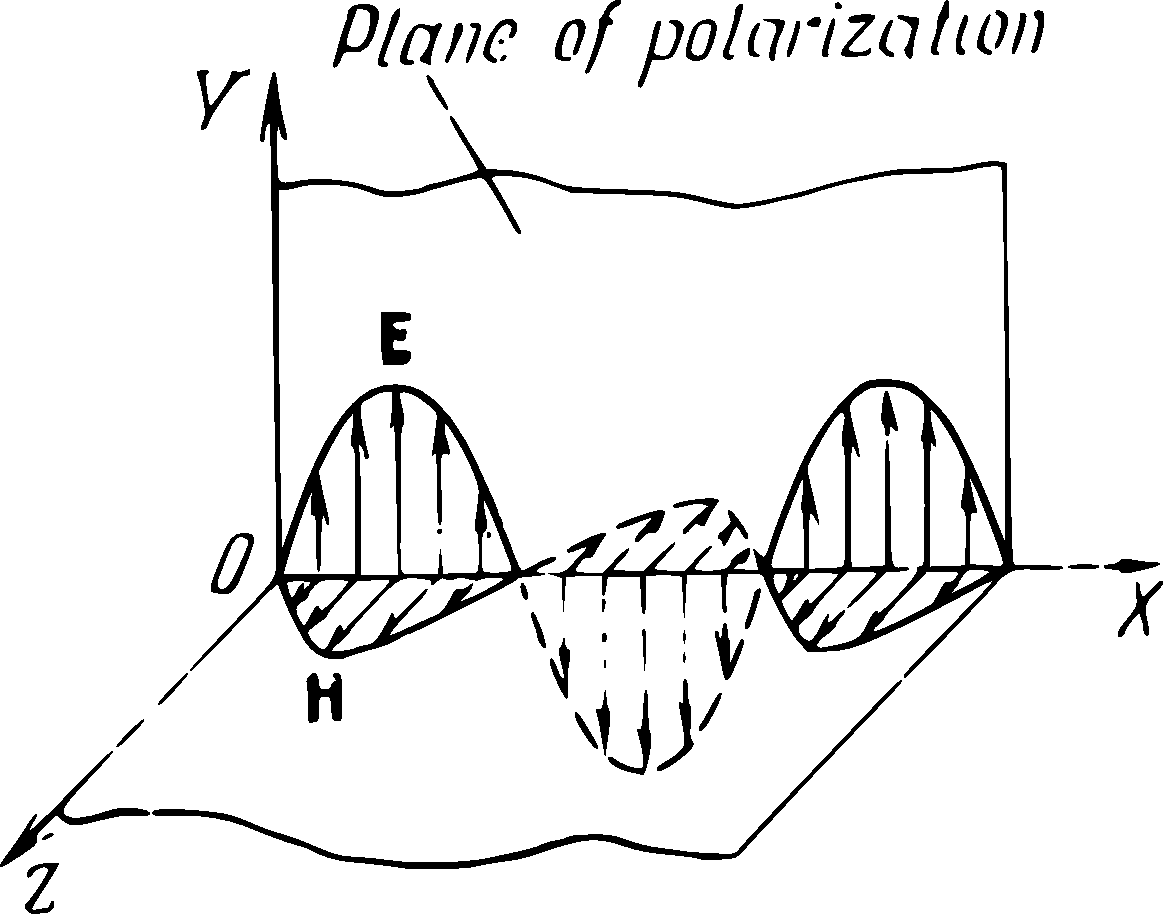
\includegraphics[width=\textwidth]{figs/ch-31/fig-31-02.pdf}
\sidecaption{Velocity vector of energy transfer by the wave.\zhcap{电磁波传递能量的速度矢量。}\label{fig-31-02}}
\end{marginfigure}

\subsection{}\label{31.1.7} For an arbitrary value of $\varphi$ \ssect{31.1.6}, a plane monochromatic wave is \redem{elliptically polarized}, i.e. at each point of the wave's field, vectors $\vb{E}$ and $\vb{H}$, while remaining mutually perpendicular,
vary with time so that their heads describe ellipses lying in a
plane perpendicular to the direction of wave propagation:
\zhpar{对于任意的 $\varphi$\ssect{31.1.6}，平面单色波是\redem{椭圆偏振}的：在波场的每一点，矢量 $\vb{E}$ 与 $\vb{H}$ 在保持相互垂直的同时随时间变化，其矢端描出位于垂直于波传播方向的平面内的椭圆：}
\begin{align*}%
\frac{E_{y}^{2}}{A_{1}^{2}} & +\frac{E_{z}^{2}}{A_{2}^{2}}  - \frac{2 E_{y}E_{z}}{A_{1}A_{2}} \cos \varphi = \sin^{2} \varphi, \qand \\
\frac{H_{y}^{2}}{A_{2}^{2}} & +\frac{H_{z}^{2}}{A_{1}^{2}}  - \frac{2 H_{y}H_{z}}{A_{1}A_{2}} \cos \varphi = \frac{\varepsilon_{r} \varepsilon_{0}}{\mu_{r} \mu_{0}} \, \sin^{2} \varphi.
\end{align*}
In particular, when $A_{1} = A_{2}$ and $\varphi = \pm (2m + 1) \pi/2$, where $m = 0, \,1,\, 2,\,\ldots{\,}$ the ellipses become circles:
\zhpar{特别地，当 $A_{1} = A_{2}$ 且 $\varphi = \pm (2m + 1) \pi/2$（其中 $m = 0, \,1,\, 2,\,\ldots{\,}$）时，椭圆变为圆：}
\begin{equation*}%
E_{y}^{2} + E_{z}^{2} = A_{1}^{2} \qand  H_{y}^{2} + H_{z}^{2} = \frac{\varepsilon_{r} \varepsilon_{0}}{\mu_{r} \mu_{0}} A_{1}^{2}.
\end{equation*}
Such a wave is said to be \redem{circularly polarized}.
\zhpar{这样的波称为\redem{圆偏振}波。}



When $\varphi = \pm m \pi$ , where $m = 0,\, 1,\, 2,\, \ldots{\,}$, the ellipses degenerate into straight lines:
\zhpar{当 $\varphi = \pm m \pi$（其中 $m = 0,\, 1,\, 2,\, \ldots{\,}$）时，椭圆退化为直线：}
\begin{equation*}%
\frac{E_{y}}{A_{1}} + \frac{E_{z}}{A_{2}}= 0 \qand \frac{H_{y}}{A_{2}} + \frac{H_{z}}{A_{2}}= 0.
\end{equation*}
Such a wave is said to be \redem{linearly}, or \redem{plane, polarized}. Shown in \figr{fig-31-02} are the values of $ a\vb{E}$ and $\vb{H}$ of the field of a plane, linearly polarized, monochromatic wave at various points along the ray ($OX$ axis) at the same instant of time. Axes $OY$ and $OZ$ are in the directions of oscillation of vectors $\vb{E}$ and $\vb{H}$, respectively, so that $E_{z} = H_{y} = 0$. 
\zhpar{这样的波称为\redem{线偏振}（或\redem{平面偏振}）波。如\figr{fig-31-02}所示，为平面线偏振单色波在同一时刻沿射线（$OX$ 轴）各点处场矢量 $ a\vb{E}$ 与 $\vb{H}$ 的值。坐标轴 $OY$ 与 $OZ$ 分别沿矢量 $\vb{E}$ 与 $\vb{H}$ 的振动方向，因此 $E_{z} = H_{y} = 0$。}

According to accepted  terminology, the plane passing through the electric vector $\vb{E}$ and the ray is called the \redem{plane of polarization} of the linearly polarized wave. Previously, this plane was called the plane of \redem{wave oscillation}, and the plane of polarization was called the one passing through the magnetic vector $\vb{H}$ and the ray (this obsolete terminology may still be found in the literature).
\zhpar{根据通用术语，包含电矢量 $\vb{E}$ 与射线的平面称为线偏振波的\redem{偏振面}。以前，该平面称为\redem{波振动面}，而将包含磁矢量 $\vb{H}$ 与射线的平面称为偏振面（这一过时的术语在一些文献中仍可能见到）。}


\subsection{}\label{31.1.8} An arbitrary plane monochromatic wave can be represented as a combination of two plane monochromatic waves of the same frequency as the first wave and simultaneously propagating in the same direction as the first wave, but linearly polarized in mutually perpendicular planes. For example, a plane monochromatic wave, propagating along the $OX$ axis \ssect{31.1.6} can be dealt with as the result of superposition of a
$y$-wave ($\vb{E}_{1} = \vb{E}_{y}$) and a $z$-wave $(\vb{E}_{2} = \vb{E}_{z})$.
\zhpar{任意平面单色波都可以表示为两个频率与原波相同、传播方向也相同、但偏振面相互垂直的线偏振平面单色波的叠加。例如，沿 $OX$ 轴传播的平面单色波\ssect{31.1.6}，可看作 $y$ 波（$\vb{E}_{1} = \vb{E}_{y}$）与 $z$ 波（$\vb{E}_{2} = \vb{E}_{z}$）的叠加。}


\section{Energy of Electromagnetic Waves}
\label{sec-31.2} 
\zhtitle{电磁波的能量}

\subsection{}\label{31.2.1} The \redem{volume energy density of an electromagnetic field} in an isotropic medium is
\zhpar{各向同性介质中\redem{电磁场的体积能量密度}为}
\begin{equation*}%
E^{d} = \frac{\varepsilon_{r} \varepsilon_{0}}{2}E^{2} + \frac{\mu_{r}\mu_{0}}{2} H^{2},
\end{equation*}
where $\varepsilon_{r}$ and $\mu_{r}$ are the relative permittivity (dielectric constant) and relative permeability of the medium. From the relations between the magnitudes of vectors $\vb{E}$ and $\vb{H}$ of the field set up by an electromagnetic wave \ssect{31.1.5} it follows that the volume energy density of electromagnetic waves is equal to
\zhpar{式中 $\varepsilon_{r}$ 与 $\mu_{r}$ 分别为介质的相对电容率（相对介电常量）与相对磁导率。由电磁波所建立的场中矢量 $\vb{E}$ 与 $\vb{H}$ 大小之间的关系\ssect{31.1.5}可知，电磁波的体积能量密度等于}
\begin{align*}%
E^{d} & = \varepsilon_{r} \varepsilon_{0} E^{2} = \mu_{r}\mu_{0} H^{2} = \sqrt{\varepsilon_{r} \varepsilon_{0} \mu_{r}\mu_{0}} \, EH \\
& = \frac{\varepsilon_{r}\mu_{r}}{c} EH,
\end{align*}
where $c$ is the velocity of electromagnetic waves in free spaee
\ssect{31.1.3}.
\zhpar{式中 $c$ 为自由空间中电磁波的速度\ssect{31.1.3}。}

\subsection{}\label{31.2.2} In the case of a plane, linearly polarized, monochromatic wave, propagating along the positive direction of axis $OX$, the field strength $E = A \sin (\omega t - kx)$. Consequently, the volume energy density of this wave is
\zhpar{对于沿 $OX$ 轴正方向传播的平面线偏振单色波，电场强度为 $E = A \sin (\omega t - kx)$。因此，该波的体积能量密度为}
\begin{equation*}%
E^{d} = \varepsilon_{r} \varepsilon_{0} A^{2} \sin^{2} (\omega t - kx).
\end{equation*}
The value of $E^{d}$ at each point of this field varies periodically with the frequency $\omega /\pi$ in a range from 0 to $E^{d}_{max} = \varepsilon_{r} \varepsilon_{0}A^{2}$.
\zhpar{在该场的每一点，$E^{d}$ 以频率 $\omega /\pi$ 周期性地变化，其取值范围为从 $0$ 到 $E^{d}_{max} = \varepsilon_{r} \varepsilon_{0}A^{2}$。}

The average value of $E^{d}$ over one period is proportional to the square of the amplitude of the field strength:
\zhpar{$E^{d}$ 在一个周期内的平均值与场强振幅的平方成正比：}
\begin{equation*}%
\expval{E^{d}} = \frac{\omega}{\pi} \int_{0} E^{d} \, \dd t = \frac{1}{2} \varepsilon_{r} \varepsilon_{0} A^{2}.
\end{equation*}
If the plane monochromatic wave has an arbitrary (elliptical)
polarization \ssect{31.1.7}, then, according to \ssect{31.1.8},
\zhpar{若平面单色波具有任意（椭圆）偏振\ssect{31.1.7}，则根据\ssect{31.1.8}，有}
\begin{align*}%
E^{d} & = \varepsilon_{r} \varepsilon_{0} [A_{1}^{2} \sin^{2} (\omega t - kx) + A_{2}^{2} \sin^{2}(\omega t - kx + \varphi)] \qand \\
\expval{E^{d}} & = \frac{1}{2} \varepsilon_{r} \varepsilon_{0} (A_{1}^{2} + A_{2}^{2}).
\end{align*}

\subsection{}\label{31.2.3} The energy flux density vector \ssect{30.3.5} of an electromagnetic
wave is called the \redem{Umov-Poynting} vector $\vb{P}$ (more
frequently, it is called the \redem{Poynting vector}). The velocity of energy transfer by a monochromatic wave is equal to the phase velocity $v = c\sqrt{\varepsilon_{r}\mu_{r}}$ of this wave \ssect{30.3.5}. Therefore, the Umov-Poynting vector for such a wave is
\zhpar{电磁波的能流密度矢量\ssect{30.3.5}称为\redem{乌莫夫-坡印廷矢量} $\vb{P}$（通常简称为\redem{坡印廷矢量}）。单色波的能量传递速度等于该波的相速度 $v = c\sqrt{\varepsilon_{r}\mu_{r}}$\ssect{30.3.5}。因此，此类波的乌莫夫-坡印廷矢量为}
\begin{equation*}%
\vb{P} = E^{d} \vb{v} = [\vb{E}\cdot \vb{H}]
\end{equation*}
In the case of a plane, lintirly polarized, monochromatic wave \ssect{31.2.2} the Umov-Poynting vector is in the direction of wave propagation and is numerically equal to
\zhpar{对于平面线偏振单色波\ssect{31.2.2}，乌莫夫-坡印廷矢量沿波的传播方向，其数值为}
\begin{equation*}%
P = \sqrt{\frac{\varepsilon_{r} \varepsilon_{0} }{\mu_{r}\mu_{0}}} A^{2} \sin^{2} (\omega t = kx).
\end{equation*}
When a plane monochromatic wave is elliptically polarized
\ssect{31.1.7},
\zhpar{当平面单色波为椭圆偏振时\ssect{31.1.7}，有}
\begin{equation*}%
P = \sqrt{\frac{\varepsilon_{r} \varepsilon_{0} }{\mu_{r}\mu_{0}}} [A_{1}^{2} \sin^{2} (\omega t - kx) + A_{2}^{2} \sin^{2}(\omega t - kx + \varphi)].
\end{equation*}

\subsection{}\label{31.2.4} The \redem{intensity $I$ of an electromagnetic wave} is a physical quantity numerically equal to the energy transferred by the wave in unit time through unit area of a surface located perpendicular to the direction of wave propagation. The intensity of an electromagnetic wave is equal to the absolute value of the average Umov-Poynting vector during a period of its complete oscillation:
\zhpar{\redem{电磁波的强度} $I$ 是一个物理量，其数值等于单位时间内通过垂直于波传播方向的单位面积的表面所传递的能量。电磁波的强度等于乌莫夫-坡印廷矢量在其完整振荡周期内平均值的绝对值：}
\begin{equation*}%
I = \abs{\expval{{P}}}.
\end{equation*}
The intensity of a travelling monochromatic wave is
\zhpar{行波单色波的强度为}
\begin{equation*}%
I = \abs{\expval{\vb{E^{d}}}}\, v,
\end{equation*}
where $v$ is the phase velocity of the wave, and $\expval{E^{d}}$ is the average value of the volume energy density of the field of the wave. The intensity of a plane, linearly polarized, travelling monochromatic wave \ssect{31.2.2} is proportional to the square of the amplitude $A$ of oscillation of the wave's field strength vector $\vb{E}$.
Thus
\zhpar{式中 $v$ 为波的相速度，$\expval{E^{d}}$ 为波场体积能量密度的平均值。平面线偏振行波单色波\ssect{31.2.2}的强度与其场强矢量 $\vb{E}$ 振幅 $A$ 的平方成正比。由此可得：}
\begin{equation*}%
I = \frac{1}{2} \sqrt{\frac{\varepsilon_{r} \varepsilon_{0}}{ \mu_{r}\mu_{0}}} \, A^{2}.
\end{equation*}
When a plane monochromatic wave is elliptically polarized
\ssect{31.1.7}, its intensity is equal to the sum of the intensities of the $y$- and $z$-waves that form the wave being considered \ssect{31.1.8}:
\zhpar{当平面单色波为椭圆偏振时\ssect{31.1.7}，其强度等于构成该波的 $y$ 波与 $z$ 波强度之和\ssect{31.1.8}：}
\begin{equation*}%
I =  I_{y} + I_{z} = \frac{1}{2} \sqrt{\frac{\varepsilon_{r} \varepsilon_{0}}{ \mu_{r}\mu_{0}}} \, (A_{1}^{2} + A_{2}^{2}).
\end{equation*}
\textbf{Note.} The \redem{intensity of light}, i.e. the electromagnetic waves dealt with in optics, is commonly understood to be the square of the amplitude of oscillation of the light wave's field strength vector $\vb{E}$.
\zhpar{\textbf{注：}\redem{光的强度}，即光学中所研究的电磁波的强度，通常理解为光波场强矢量 $\vb{E}$ 振幅的平方。}

\subsection{}\label{31.2.5} The intensity $I$ of a spherical, linearly polarized, monochromatic wave is related to the amplitude $A$ of oscillation of vector $\vb{E}$ in the same way as for a plane wave \ssect{31.2.4}. But the amplitude and intensity of a spherical wave decrease as the distance $r$ increases from the wave centre \ssect{30.3.6}:
\zhpar{球面线偏振单色波的强度 $I$ 与矢量 $\vb{E}$ 振动振幅 $A$ 之间的关系，与平面波相同\ssect{31.2.4}。但球面波的振幅和强度都随距波源中心的距离 $r$ 增大而减小\ssect{30.3.6}：}
\begin{equation*}%
A = \frac{a_{0}}{r} \qand I = \frac{i_{0}}{r^{2}}.
\end{equation*}

\subsection{}\label{31.2.6} Electromagnetic waves exert pressure on the obstacles in their path that absorb and reflect the waves. The \redem{pressure of electromagnetic waves} is explained by the fact that due to the effect of the waves' electric field charged particles of matter are put into ordered motion and are subject to the action of Lorentz forces exerted by the magnetic field \ssect{24.1.1}.
\zhpar{电磁波会对其路径上吸收和反射电磁波的障碍物施加压强。\redem{电磁波的压强}可解释为：由于电磁波电场的作用，物质中的带电粒子被驱动做有序运动，并受到磁场施加的洛伦兹力的作用\ssect{24.1.1}。}

According to Maxwell's theory the pressure of electromagnetic
waves is equal to
\zhpar{按照麦克斯韦理论，电磁波的压强等于}
\begin{equation*}%
p = \frac{I}{v} (1 + R) \cos^{2} i = \expval{E^{d}} (1 + R) \cos^{2} i,
\end{equation*}
where $I$ is the intensity of the wave incident on the obstacle,
$v$ is its velocity, $\expval{E^{d}}$ is the average value of the volume energy density of the wave, $i$ is the angle of incidence \ssect{31.5.2}, and $R$ is the reflection coefficient \ssect{31.5.6}.
\zhpar{式中 $I$ 为入射到障碍物上的波的强度，$v$ 为其速度，$\expval{E^{d}}$ 为波的体积能量密度的平均值，$i$ 为入射角\ssect{31.5.2}，$R$ 为反射系数\ssect{31.5.6}。}

\section{Electromagnetic Radiation}
\label{sec-31.3} 
\zhtitle{电磁辐射}


\subsection{}\label{31.3.1} The process of exciting electromagnetic waves and emitting them into surrounding space by some system is called the \redem{radiation} of these \redem{waves}. The system itself is called the \redem{radiating
system}. The field set up by these electromagnetic waves is called the \redem{radiation field}. According to the concepts of classical electrodynamics, electromagnetic waves are excited by electric charges travelling with acceleration (in particular, an electric circuit in which the current varies). Vavilov-Cherenkov radiation can also occur in matter \ssect{34.6.1}.
\zhpar{某一系统激发电磁波并将其发射到周围空间的过程，称为这些\redem{波}的\redem{辐射}。该系统称为\redem{辐射系统}，由这些电磁波建立的场称为\redem{辐射场}。根据经典电动力学的概念，电磁波由做加速运动的电荷（特别是电流随时间变化的电路）激发。在物质中也可能发生瓦维洛夫-切伦科夫辐射\ssect{34.6.1}。}

The simplest radiating system is the electric dipole \ssect{15.2.3} whose dipole moment $\vb{p}_{e}$ varies with time. Such an ``oscillating'' dipole is called an \redem{oscillator}, or \redem{elementary vibrator}. Oscillators are extensively used in physics for simulating and calculating the radiation fields of real systems. If the radiating system is electrically neutral and its size is small compared to the length $\lambda$ of the waves it radiates, then in the wave zone of the system, i.e. at points whose distance from the system equals $r \gg \lambda$, the radiation field is almost the same as that of an oscillator having the same electric dipole moment as the whole radiating system.
\zhpar{最简单的辐射系统是偶极矩 $\vb{p}_{e}$ 随时间变化的电偶极子\ssect{15.2.3}。这种“振荡”偶极子称为\redem{振子}，或称\redem{基本振子}。振子在物理学中被广泛用于模拟和计算实际系统的辐射场。若辐射系统是电中性的，且其尺寸远小于它所辐射的波长 $\lambda$，则在该系统的波区内（即距离系统为 $r \gg \lambda$ 的点处），辐射场几乎与一个偶极矩等于整个辐射系统偶极矩的振子的辐射场相同。}

\subsection{}\label{31.3.2} A \redem{linear harmonic oscillator} is an electric dipole whose moment $\vb{p}_{e}$ varies according to the harmonic law:
\zhpar{\redem{线性谐振子}是指其偶极矩 $\vb{p}_{e}$ 按简谐规律变化的电偶极子：}
\begin{equation*}%
\vb{p}_{e} = \vb{p}_{0} \sin \omega t \text{  where  } \vb{p}_{0} = \text{const}.
\end{equation*}
At point $M$ of the wave zone of a linear harmonic oscillator,
located in vacuum, the vectors $\vb{E}$ and $\vb{H}$ of the radiation field at the instant of time t are equal to:
\zhpar{位于真空中的线性谐振子波区内的点 $M$ 处，在时刻 $t$ 辐射场的矢量 $\vb{E}$ 与 $\vb{H}$ 为：}
\begin{align*}%
\vb{E} (t) & = - \frac{\mu_{0}\omega^{2}}{4 \pi r^{3}} [[\vb{p}_{0} \cross \vb{r}]\cross \vb{r}] \sin (\omega t - kr), \\ 
\vb{H} (t) & = - \frac{\omega^{2}}{4 \pi c r^{3}} [\vb{p}_{0}  ]\cross \vb{r}] \sin (\omega t - kr), 
\end{align*}
\begin{marginfigure}%[-1.5cm]
\centering
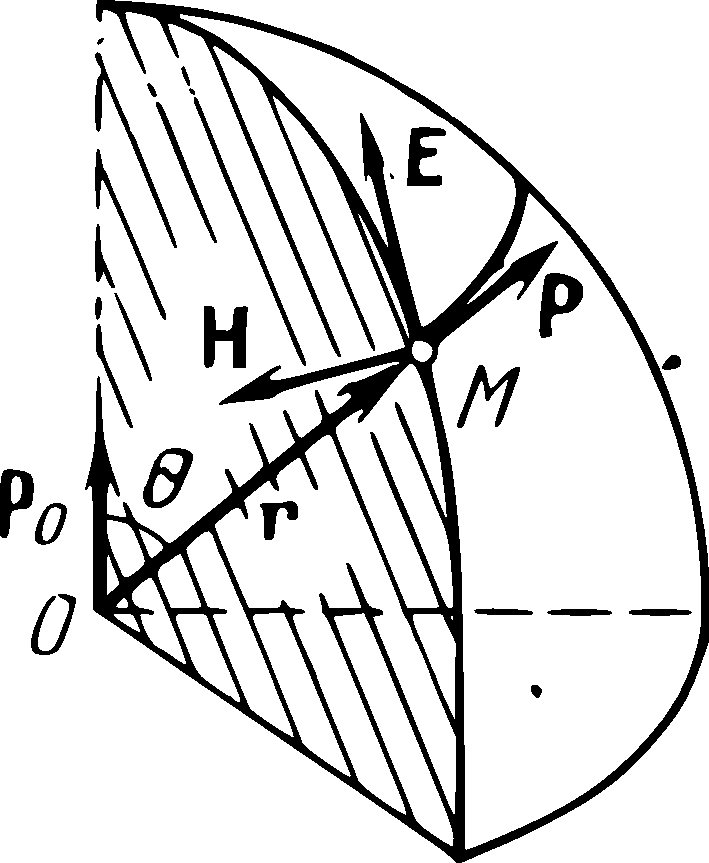
\includegraphics[width=0.7\textwidth]{figs/ch-31/fig-31-03.pdf}
\sidecaption{Orientation of $\vb{E}$, $\vb{H}$ and $\vb{r}$ form a right-hand set of three vectors.\zhcap{$\vb{E}$、$\vb{H}$ 与 $\vb{r}$ 构成右手系的三个矢量。}
 \label{fig-31-03}}
\end{marginfigure}
where $\vb{r}$ is the radius vector from point $O$, where the dipole is located, to point $M$ (\figr{fig-31-03}). Vectors $\vb{E}$ and $\vb{H}$ are mutually perpendicular and lie in a plane perpendicular to the radius vector $\vb{r}$. Hence, $\vb{E}$, $\vb{H}$ and $\vb{r}$ form a right-hand set of three vectors.
\zhpar{式中 $\vb{r}$ 为由偶极子所在点 $O$ 指向点 $M$ 的位矢（见\figr{fig-31-03}）。矢量 $\vb{E}$ 与 $\vb{H}$ 相互垂直，且都位于垂直于位矢 $\vb{r}$ 的平面内。因此，$\vb{E}$、$\vb{H}$ 与 $\vb{r}$ 构成右手系的三个矢量。}

Vector $\vb{E}$ is tangent to the meridian, and vector $\vb{H}$ is tangent to the latitudinal circle passing through point $M$ of a sphere of radius $r$ having its centre at point $O$.
\zhpar{矢量 $\vb{E}$ 与子午线相切，矢量 $\vb{H}$ 与通过点 $M$、以 $O$ 为球心、半径为 $r$ 的球面上的纬圈相切。}

\subsection{}\label{31.3.3} The Umov-Poynting vector at point $M$ of the wave zone of a linear harmonic oscillator is
\zhpar{线性谐振子波区内点 $M$ 处的乌莫夫-坡印廷矢量为}
\begin{equation*}%
\vb{P} = \frac{\mu_{0}\omega^{4}p_{0}^{2}\sin^{2} \theta}{16 \pi^{2} c r^{3}} \vb{r} \sin^{2} (\omega t - kr),
\end{equation*}
where $\theta$ is the angle between vectors $\vb{p}_{0}$ and $\vb{r}$.
\zhpar{式中 $\theta$ 为矢量 $\vb{p}_{0}$ 与 $\vb{r}$ 之间的夹角。}

\begin{marginfigure}%[-3cm]
%\centering
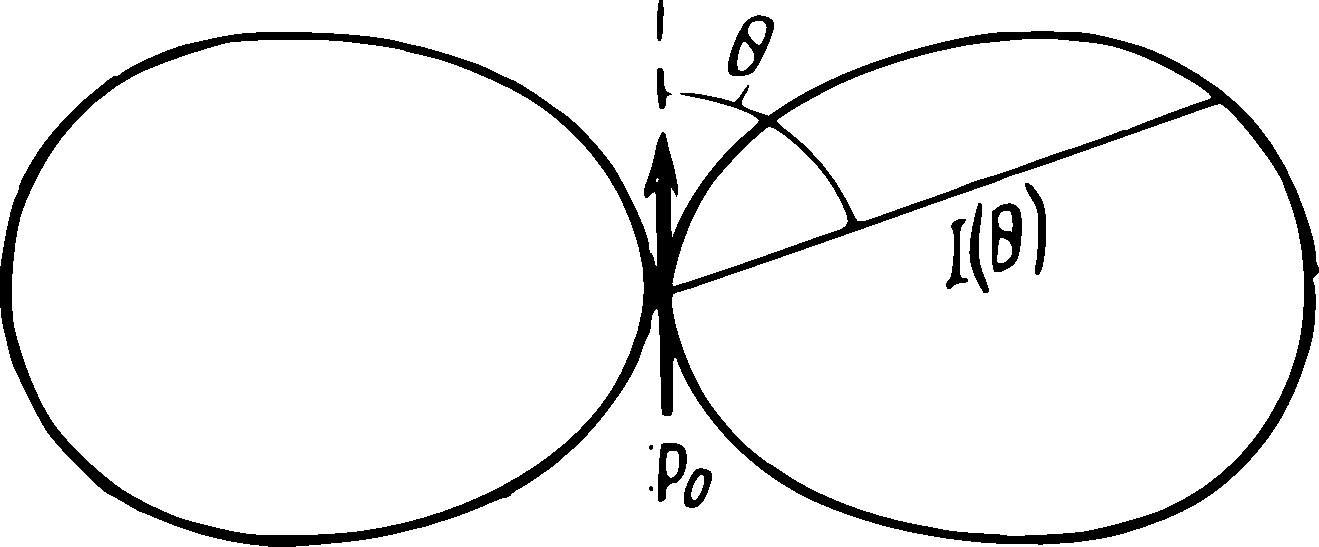
\includegraphics[width=0.8\textwidth]{figs/ch-31/fig-31-04.pdf}
\sidecaption{The dependence of $I$ on $\theta$. \zhcap{$I$ 随 $\theta$ 的变化关系。}\label{fig-31-04}}
\end{marginfigure}


The intensity of the electromagnetic wave at point $M$ is
\zhpar{点 $M$ 处电磁波的强度为}
\begin{equation*}%
I =  \frac{\mu_{0}\omega^{4}p_{0}^{2}\sin^{2} \theta}{32 \pi^{2 c r^{2}}}
\end{equation*}
The dependence of $I$ on $\theta$ for a fixed value of $r$, shown in polar coordinates (\figr{fig-31-04}), is called the \redem{polar directional diagram of oscillator (dipole) radiation}. The dipole radiates most intensively in directions that make an angle $\theta = \pi/2$ with its axis, i.e. in a plane passing through the middle of the dipole and perpendicular to its axis. Along its axis ($\theta = 0$ and $\theta = \pi$) the dipole does not radiate at all.
\zhpar{对于固定的 $r$，$I$ 随 $\theta$ 的变化关系（用极坐标表示，见\figr{fig-31-04}）称为振子（偶极子）辐射的\redem{极坐标方向图}。偶极子沿与其轴线成 $\theta = \pi/2$ 角的方向辐射最强，即在通过偶极子中点并垂直于其轴线的平面内。沿其轴线方向（$\theta = 0$ 与 $\theta = \pi$），偶极子根本不辐射。}

The average power of radiation of a linear harmonic oscillator is
\zhpar{线性谐振子的平均辐射功率为}
\begin{equation*}%
\expval{P^{r}} = 2 \pi r^{2} \int_{0}^{\pi} I \sin \theta \, \dd \theta = \frac{\mu_{0}\omega^{4} p_{0}^{2}}{12 \pi c}.
\end{equation*}


\subsection{}\label{31.3.4} The instantaneous power of radiation of charge $q$, travelling at the acceleration $\vb{a}$, is
\zhpar{以加速度 $\vb{a}$ 运动的电荷 $q$ 的瞬时辐射功率为}
\begin{equation*}%
P^{r}_{\text{ins}} = \frac{\mu_{0}}{6 \pi c} q^{2} a^{2}.
\end{equation*}
If the charge executes harmonic oscillation of the amplitude $l_{0}$ and angular frequency $\omega$, the average power of its radiation is
\zhpar{若电荷做振幅为 $l_{0}$、角频率为 $\omega$ 的简谐振动，则其辐射的平均功率为}
\begin{equation*}%
\expval{P^{r}} = \frac{\mu_{0}q^{2} \omega^{4} l_{0}^{2}}{12 \pi c}.
\end{equation*}
According to classical theory the radiation of light by atoms is due to the vibration of electrons in them. Owing to the consumption of energy to produce radiation this vibration is gradually damped, i.e. its amplitude varies according to the law
\ssect{29.1.3}: 
\zhpar{根据经典理论，原子发光是由于其中电子的振动。由于辐射要消耗能量，这种振动会逐渐衰减，即其振幅按下列规律变化\ssect{29.1.3}：}
\begin{equation*}%
l_{0} = l_{00} \exp (-\beta t)
\end{equation*}
where $l_{00}$ is the initial amplitude and $\beta$ is the damping factor. The energy of vibration of an electron \ssect{28.2.2} is
\zhpar{式中 $l_{00}$ 为初始振幅，$\beta$ 为阻尼系数。电子振动的能量\ssect{28.2.2}为}
\begin{equation*}%
 E = m_{e}\omega^{2} l_{0}^{2} /2, 
\end{equation*}
where $m_{e}$ is the mass of the electron. Since $-\dd E = \expval{P^{r}} \, \dd t = 2\beta E \, \dd t$ and $q = -e$, the
relaxation time \ssect{29.1.3} of this vibration, called the average \redem{de-excitation time of the atom}, is
\zhpar{式中 $m_{e}$ 为电子的质量。由于 $-\dd E = \expval{P^{r}} \, \dd t = 2\beta E \, \dd t$，且 $q = -e$，该振动的弛豫时间\ssect{29.1.3}（称为原子的平均\redem{退激时间}）为}
\begin{equation*}%
\tau = \frac{1}{\beta} = \frac{12 \pi c m_{e}}{\mu_{0} e^{2} \omega^{2}}.
\end{equation*}
For visible light $\omega \approx \SI{4d15}{\per\second}$ and $\tau \approx \SI{2d-8}{\per\second}$
\zhpar{对于可见光，$\omega \approx \SI{4d15}{\per\second}$，$\tau \approx \SI{2d-8}{\per\second}$。}

\section{Electromagnetic Spectrum}
\label{sec-31.4} 
\zhtitle{电磁波谱}


\subsection{}\label{31.4.1} Depending upon the frequency $nu$ (or wavelength $\lambda = c/\nu$ in vacuum, where $c$ is the velocity of electromagnetic waves in free space), as well as on the way in which they are radiated and recorded (or detected), distinction is made between several kinds of electromagnetic waves: radio waves, optical radiation, X-rays and gamma rays.
\zhpar{根据电磁波的频率 $\nu$（或真空中的波长 $\lambda = c/\nu$，其中 $c$ 为自由空间中电磁波的速度），以及其辐射和接收（或探测）的方式，可将电磁波分为若干种类：无线电波、光辐射、X射线和伽马射线。}

\redem{Radio waves} are electromagnetic waves of a length $\lambda$ in free space that exceeds \SI{5d-5}{\meter} (correspondingly, $\nu < \SI{6d12}{\hertz}$).
\zhpar{\redem{无线电波}是指自由空间中波长 $\lambda$ 超过 \SI{5d-5}{\meter} 的电磁波（相应地，$\nu < \SI{6d12}{\hertz}$）。}

In connection with special features of their propagation and
generation, the full range of radio waves is commonly divided
into nine bands (\tabl{tab-31.1}).
\zhpar{考虑到无线电波在传播和产生方面的特殊性，通常将整个无线电波范围划分为九个波段（见\tabl{tab-31.1}）。}


%\begin{small}
\begin{table*}[h]
\begin{center}
{\small
\begin{tabular}{@{}p{4.25cm}ll@{}}
\toprule
\textbf{Band Name} & \textbf{Wavelength (\si{\meter})} & \textbf{Frequency (\si{\hertz})} \\
\midrule
Very-long (myriametric) waves & Over \SI{d4}{} & Less than \SI{3e4}{} \\
Long (kilometric) waves & \SI{d4}{} to \SI{d3}{} & \SI{3e4}{} to \SI{3e5}{} \\
Medium (hectometric) waves & \SI{d3}{} to \SI{d2}{} & \SI{3e5}{} to \SI{3e6}{} \\
Short (decametric) waves & \SI{d2}{} to \SI{10}{} & \SI{3e6}{} to \SI{3e7}{} \\
Metric waves & \SI{10}{} to \SI{1}{} & \SI{3e7}{} to \SI{3e8}{} \\
Decimetric waves & \SI{1}{} to \SI{d-1}{} & \SI{3e8}{} to \SI{3e9}{} \\
Centimetric waves & \SI{d-1}{} to \SI{d-2}{} & \SI{3e9}{} to \SI{3e10}{} \\
Millimetric waves & \SI{d-2}{} to \SI{d-3}{} & \SI{3e10}{} to \SI{3e11}{} \\
Submillimetric waves & \SI{d-3}{} to \SI{d-5}{} & \SI{3e11}{} to \SI{6e12}{} \\
\bottomrule
\end{tabular}}
\sidecaption[][2cm]{Full range of radio waves divided into nine bands. \zhcap{无线电波的全部范围划分为九个波段。}\label{tab-31.1}}
\end{center}
\end{table*}
%\end{small}

%
%TABLE 31.1
%Band name Wavelength, m Frequency, Hz
%Very-long (myria- Over 104 Less than 3 X 10*
%metric) waves
%Long (kilometric)
%104 to 103 3 x 104 to 3 x 105
%waves
%Medium (hecto-
%103 to 102 3 x 105 to 3 X 10®
%metric) waves
%Short (decametric)
%102 to 10 3 x 10® to 3 X 107
%waves
%Metric waves 10 to 1 3 x 107 to 3 X 108
%Decimetric waves 1 to 0.1 3 x 108 to 3 x 10°
%Centime trie waves 0.1 to 0.01 3 x 10« to 3 x 1010
%Millimetric waves 10"2 to 10-3 3 X 10w to 3 x 1011
%Submillimetric
%103 to 5 X 10"5 3 X 1011 to 6 X 1012
%waves

\subsection{}\label{31.4.2} Radio frequencies are divided into twelve bands according to the international regulations for radio communications. These bands and their corresponding wavelength in free space are listed in Table 31.2.
\zhpar{根据国际无线电通信规则，射频共分为十二个波段。这些波段及其在自由空间中对应的波长列于表 31.2 中。}

%\begin{small}
\begin{table*}%[H]
\centering
{\small
\begin{tabular}{@{}p{1.25cm}p{2.25cm}p{2.75cm}p{2.25cm}p{2.75cm}@{}}
\toprule
\textbf{Band No.} & \textbf{Frequency\newline Band} & \textbf{Designation} & \textbf{Wavelength \newline Band} & \textbf{Wave \newline Designation} \\
\midrule
Band 1 & \SI{3}{\hertz} to \SI{30}{\hertz} & Extremely Low Frequency (ELF) & \SI{100}{\mega\meter} to \SI{10}{\mega\meter} & Dekamegametric waves\\
Band 2 & \SI{30}{\hertz} to \SI{300}{\hertz} & Super Low Frequency (SLF) & \SI{10}{\mega\meter} to \SI{1}{\mega\meter} & Megametric waves\\
Band 3 & \SI{0.3}{\kilo\hertz} to \SI{3}{\kilo\hertz} & Voice Frequency (VF) & \SI{1000}{\kilo\meter} to \SI{100}{\kilo\meter} & Hectokilometric waves\\
Band 4 & \SI{3}{\kilo\hertz} to \SI{30}{\kilo\hertz} & Very Low Frequency (VLF) & \SI{100}{\kilo\meter} to \SI{10}{\kilo\meter} & Myriametric waves\\
Band 5 & \SI{30}{\kilo\hertz} to \SI{300}{\kilo\hertz} & Low Frequency (LF) & \SI{10}{\kilo\meter} to \SI{1}{\kilo\meter} & Kilometric waves\\
Band 6 & \SI{0.3}{\mega\hertz} to \SI{3}{\mega\hertz} & Medium Frequency (MF) & \SI{1}{\kilo\meter} to \SI{0.1}{\kilo\meter} & Hectometric waves\\
Band 7 & \SI{3}{\mega\hertz} to \SI{30}{\mega\hertz} & High Frequency (HF) & \SI{100}{\meter} to \SI{10}{\meter} & Dekametric waves\\
Band 8 & \SI{30}{\mega\hertz} to \SI{300}{\mega\hertz} & Very High Frequency (VHF) & \SI{10}{\meter} to \SI{1}{\meter} & Metric Frequency \\
Band 9 & \SI{0.3}{\giga\hertz} to \SI{3}{\giga\hertz} & Ultra High Frequency (UHF) & \SI{1}{\meter} to \SI{0.1}{\meter} & Decimetric waves\\
Band 10 & \SI{3}{\giga\hertz} to \SI{30}{\giga\hertz} & Super High Frequency (SHF) & \SI{10}{\centi\meter} to \SI{1}{\centi\meter} & Centimetric waves\\
Band 11 & \SI{30}{\giga\hertz} to \SI{300}{\giga\hertz} & Extremely High Frequency (EHF) & \SI{10}{\milli\meter} to \SI{1}{\milli\meter} & Millimetric waves\\
Band 12 & \SI{0.3}{\tera\hertz} to \SI{3}{\tera\hertz} & Hyper High Frequency (HHF) & \SI{1}{\milli\meter} to \SI{0.1}{\milli\meter} & Decimillimetric waves\\
\bottomrule
\end{tabular}}
\sidecaption[][4cm]{Radio-frequency band designations with corresponding frequency and wavelength ranges. Note: In the terminology accepted in the U.S.A. the extremely low frequency (ELF) band includes frequencies from \SI{3}{\hertz}
\SI{3}{\kilo\hertz}, i.e. the first three bands of the list given here.\zhcap{射频波段的划分及其对应的频率与波长范围。注：按美国术语，极低频（ELF）波段包括从 \SI{3}{\hertz} 到 \SI{3}{\kilo\hertz} 的频率，即本表中前三个波段。}\label{tab-31.2}}
\end{table*}
%\end{small}
%
%TABLE 31.2
%Radio-frequency band designation
%Band limits
%Radio-wave band designation
%Band limits
%Basic designation
%Optional designation
%Basic designation
%Optional dasignation
%Band 1
%Extremely low fre- ELF
%3 to 30 Hz
%Band 1
%Dekamegametric
%100 to 10 Mm
%quency *
%waves
%Band 2
%Super
%low fre- SLF
%quency
%30 to 300 Hz
%Band 2
%Megametric waves
%10 to 1 Mm
%Band 3
%Voice frequency
%VF
%0.3 to 3 kHz
%Band 3
%Hectokilometric
%1000 to 100 km
%Band 4
%Very low fre-
%VLF
%quency
%3 to 30 kHz
%Band 4
%waves
%Myriametric waves
%100 to 10 km
%Band 5
%Low frequency
%LF
%30 to 300 kHz
%Band 5
%Kilometric waves
%10 to 1 km
%Band 6
%Medium frequency
%MF
%0.3 to 3 MHz
%Band 6
%Hectometric waves 1 to 0.1 km
%
%Band 7
%High frequency
%HF
%3 to 30 MHz
%Band 7
%Dekametric waves
%100 to 10 m
%Band 8
%Very
%high
%quency
%fre- VHF
%30 to 300 MHz
%Band 8
%Metric waves
%10 to 1 m
%ELECTROMAGNETIC
%Band 9
%UItra
%high fre- UHF
%quency
%0.3 to 3 GHz
%Band 9
%Decimetric waves
%1 to 0.1 m
%Band 10
%Super high
%fre- SHF
%quency
%3 to 30 GHz
%
%Band 10 Centimetric waves 10 to 1 cm
%
%Band 11
%Extremely
%high EHF
%frequency
%30 to 300 GHz
%
%Band 11 Millimetric
%waves
%10 to 1 mm
%
%Band 12 Hyper high fre- HHF
%quency
%0.3 to 3 THz
%Band 12
%Decimillimetric waves
%1 to 0.1 mm
%WAVES



\subsection{}\label{31.4.3} \redem{Optical radiation}, or \redem{light}, refers to electromagnetic waves
(electromagnetic radiation) of a wavelength in vacuum ranging
from \SI{10}{\nano\meter} to \SI{1}{\milli\meter} (by convention). Optical radiation includes infrared, visible and ultraviolet radiation.\sidenote{According to the recommendation of the Committee for Scientific and Engineering Terminology of the USSR Academy of Sciences [Physical Optics (Terminology), Collection of Recommended Terms, Issue 74, Nauka Publishers, 1968, Moscow] optical radiation also includes X-rays, the range of wavelengths of optical radiation being established from \SI{0.1}{\angstrom} (\SI{d-11}{\nano\meter}) to \SI{1}{\centi\meter}.}
\zhpar{\redem{光辐射}，或称\redem{光}，是指真空中波长（按惯例）从 \SI{10}{\nano\meter} 到 \SI{1}{\milli\meter} 的电磁波（电磁辐射）。光辐射包括红外辐射、可见光和紫外辐射。}
\zhpar{注：根据苏联科学院科学与工程术语委员会的建议（《物理光学（术语）》，推荐术语汇编第 74 期，Nauka 出版社，1968 年，莫斯科），光辐射还包括 X 射线，光辐射的波长范围规定为从 \SI{0.1}{\angstrom}（\SI{d-11}{\nano\meter}）到 \SI{1}{\centi\meter}。}

\redem{Infrared (IR) radiation} is the electromagnetic radiation emitted by heated bodies. Its wavelength in vacuum is within the range from \SI{1}{\milli\meter} to \SI{770}{\nano\meter} (\SI{1}{\nano\meter} = \SI{d-9}{\meter}).
\zhpar{\redem{红外（IR）辐射}是由受热物体发出的电磁辐射，其真空中的波长范围为从 \SI{1}{\milli\meter} 到 \SI{770}{\nano\meter}（\SI{1}{\nano\meter} = \SI{d-9}{\meter}）。}

\redem{Visible radiation}, or \redem{visible light}, is electromagnetic radiation of a wavelength in vacuum from \SI{770}{\nano\meter} to \SI{380}{\nano\meter}. It is capable of directly producing a visible sensation in the human eye.
\zhpar{\redem{可见辐射}，或称\redem{可见光}，是真空中波长为 \SI{770}{\nano\meter} 至 \SI{380}{\nano\meter} 的电磁辐射。它能够直接在人眼中引起可见的感觉。}

\redem{Ultraviolet (UV) radiation} is electromagnetic radiation of a wavelength in vacuum from \SI{300}{\nano\meter} to \SI{10}{\nano\meter}.
\zhpar{\redem{紫外（UV）辐射}是真空中波长为 \SI{300}{\nano\meter} 至 \SI{10}{\nano\meter} 的电磁辐射。}

\subsection{}\label{31.4.4} \redem{X-radiation}, or \redem{X-rays} (also called \redem{Roentgen rays}), is the electromagnetic radiation produced in the interaction of charged
particles and photons \ssect{37.1.4} with atoms of matter. Its wavelength in vacuum ranges within the wide conditional limits
from \SI{10}{\nano\meter} or \SI{100}{\nano\meter} to \SI{d-2}{\pico\meter} or \SI{1}{\pico\meter} (\SI{1}{\pico\meter} = \SI{d-12}{\meter}).
\zhpar{\redem{X辐射}，或称\redem{X射线}（又称\redem{伦琴射线}），是带电粒子和光子\ssect{37.1.4}与物质原子相互作用时产生的电磁辐射。其真空中的波长在较宽的条件范围内变化，从 \SI{10}{\nano\meter} 或 \SI{100}{\nano\meter} 到 \SI{d-2}{\pico\meter} 或 \SI{1}{\pico\meter}（\SI{1}{\pico\meter} = \SI{d-12}{\meter}）。}

\redem{Gamma radiation}, or \redem{gamma rays}, is electromagnetic radiation of a wavelength in vacuum less than \SI{d-1}{\nano\meter}. It is emitted by excited atomic nuclei upon radioactive transformations and nuclear reactions. It is also formed in particle decay, in particle-antiparticle, annihilation \ssect{43.5.5} and other processes.
\zhpar{\redem{伽马辐射}，或称\redem{伽马射线}，是真空中波长小于 \SI{d-1}{\nano\meter} 的电磁辐射。它由激发态原子核在放射性衰变和核反应中发出，也在粒子衰变、粒子-反粒子湮灭\ssect{43.5.5}以及其他过程中产生。}

\section[Reflection and Refraction]{Reflection and Refraction of Electromagnetic Waves at the Interface Between Two Dielectric Media}
\label{sec-31.5} 
\zhtitle{电磁波在两种电介质分界面上的反射和折射}




\subsection{}\label{31.5.1} The \redem{refractive index (absolute refractive index) of a medium} is the quantity $n$, which is equal to the ratio of the velocity $c$
of the electromagnetic waves in vacuum to their phase velocity
$v$ in the medium: $n = c/v$. From \ssect{31.1.3} it follows that $n = \sqrt{\varepsilon_{r}\mu_{r}}$, where $\varepsilon_{r}$ and $\mu_{r}$ are the relative dielectric permittivity
and relative magnetic permeability of the medium.
\zhpar{\redem{介质的折射率}（绝对折射率）是一个量 $n$，它等于真空中电磁波的速度 $c$ 与该介质中相速度 $v$ 之比：$n = c/v$。由\ssect{31.1.3}可知 $n = \sqrt{\varepsilon_{r}\mu_{r}}$，其中 $\varepsilon_{r}$ 与 $\mu_{r}$ 分别为介质的相对电容率与相对磁导率。}

For media having no ferromagnetic properties, $\mu_{r} \approx  1$ and $n \approx \varepsilon_{r}$.
\zhpar{对于不具有铁磁性的介质，$\mu_{r} \approx 1$，$n \approx \varepsilon_{r}$。}

The \redem{relative refractive index of two} media (of the second medium with respect to the first) is the quantity $n_{21}$, equal to the ratio of the refractive indices of these media: $n_{21} = n_{2}/n_{1}$. For non-ferromagnetic
media $n_{21} = \sqrt{\varepsilon_{r2}/\varepsilon_{r1}}.$
\zhpar{两种介质的\redem{相对折射率}（第二种介质相对于第一种介质）是一个量 $n_{21}$，它等于两种介质折射率之比：$n_{21} = n_{2}/n_{1}$。对于非铁磁性介质，$n_{21} = \sqrt{\varepsilon_{r2}/\varepsilon_{r1}}$。}

\begin{marginfigure}[-1.5cm]
\centering
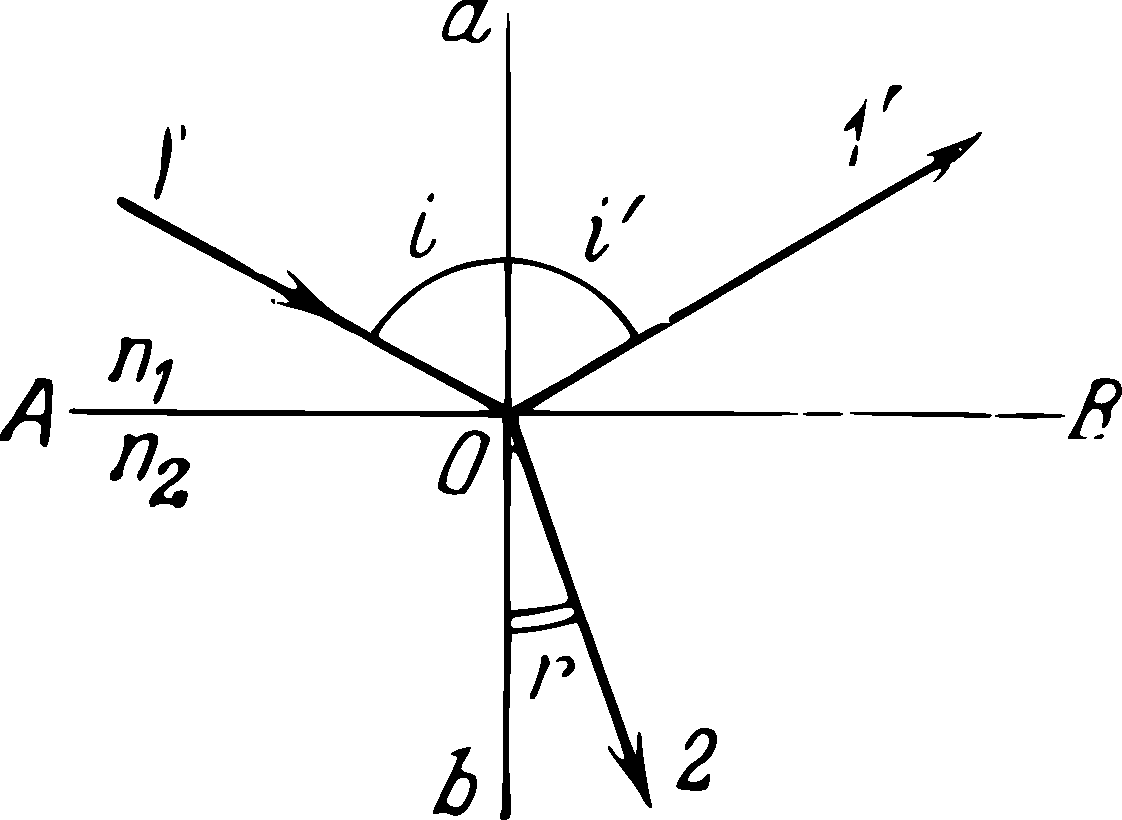
\includegraphics[width=\textwidth]{figs/ch-31/fig-31-05.pdf}
\sidecaption{Reflection and refraction of a wave at the interface between two media.\zhcap{波在两种介质分界面上的反射与折射。}\label{fig-31-05}}
\end{marginfigure}

\subsection{}\label{31.5.2} When an electromagnetic wave falls on the interface between two media, it is partly reflected from the interface and partly refracted as it enters the second medium. 
\zhpar{电磁波入射到两种介质的分界面上时，一部分在分界面上被反射，另一部分在进入第二种介质时发生折射。}

In \figr{fig-31-05} the line $AB$ is the plane interface between
the media. Rays $\mathit{1}$, $\mathit{1'}$ and $\mathit{2}$ represent the directions of propagation of the incident, reflected and refracted plane waves. They are called the \redem{incident}, \redem{reflected} and \redem{refracted rays}, respectively, and the angles between them and the angles they make with the perpendicular ab to the interface at the point of incidence $O$ are: $i$ is the \redem{angle of incidence}, $i'$ is the \redem{angle of reflection} and $r$ is the \redem{refractive angle}.
\zhpar{如\figr{fig-31-05}所示，直线 $AB$ 为两种介质之间的平面分界面。射线 $\mathit{1}$、$\mathit{1'}$ 与 $\mathit{2}$ 分别表示入射平面波、反射平面波与折射平面波的传播方向，它们分别称为\redem{入射线}、\redem{反射线}与\redem{折射线}。它们之间的夹角，以及它们与入射点 $O$ 处分界面的垂线 ab 所成的夹角分别为：$i$ 为\redem{入射角}，$i'$ 为\redem{反射角}，$r$ 为\redem{折射角}。}

The \redem{plane of incidence} is the plane passing through the incident ray and perpendicular to the interface at the point of incidence.
\zhpar{\redem{入射面}是指通过入射线并垂直于入射点处分界面的平面。}

\subsection{}\label{31.5.3} The laws of reflection and refraction of electromagnetic waves at the interface between two dielectric media can be obtained on the basis of the boundary conditions for an electromagnetic field \ssect{27.4.4}. In the first medium the field of the reflected wave ($\vb{E}^{\text{rfl}}$ and $\vb{H}^{\text{rfl}}$) is superposed on the field of the incident wave ($\vb{E}^{0}$ and $\vb{H}^{0}$). In the second medium there is only the field ($\vb{E}^{\text{rfr}}$ and $\vb{H}^{\text{rfr}}$) of the refracted wave (propagating in this medium). Hence, the boundary conditions are of the form (assuming that $\mu_{r2} = \mu_{r1} = 1$):
\zhpar{电磁波在两种电介质分界面上的反射和折射定律，可由电磁场的边界条件\ssect{27.4.4}导出。在第一种介质中，反射波的场（$\vb{E}^{\text{rfl}}$ 与 $\vb{H}^{\text{rfl}}$）与入射波的场（$\vb{E}^{0}$ 与 $\vb{H}^{0}$）相叠加。在第二种介质中，只有折射波（在该介质中传播）的场（$\vb{E}^{\text{rfr}}$ 与 $\vb{H}^{\text{rfr}}$）。因此，边界条件的形式为（假设 $\mu_{r2} = \mu_{r1} = 1$）：}
\begin{align*}%
E_{\tau}^{0} + E_{\tau}^{\text{rfl}} & = E_{\tau}^{\text{rfr}}, & \quad \varepsilon_{r1} (E_{n}^{0} + E_{n}^{\text{rfl}}) & = \varepsilon_{r2} E_{n}^{\text{rfr}},\\
H_{\tau}^{0} + H_{\tau}^{\text{rfl}} & = H_{\tau}^{\text{rfr}}, & \quad (H_{n}^{0} + H_{n}^{\text{rfl}}) & = H_{n}^{\text{rfr}}.
\end{align*}
Here $E_{\tau}$, $H_{\tau}$, $E_{n}$ and $H_{n}$ are the projections of vectors $\vb{E}$ and $\vb{H}$ on the tangential plane and the normal to the interface between the media. It follows from these relations that in the incidence of a plane monochromatic wave on a smooth plane interface between media, the following laws are complied with (regardless of the kind of polarization of this wave):
\zhpar{其中 $E_{\tau}$、$H_{\tau}$、$E_{n}$ 与 $H_{n}$ 分别为矢量 $\vb{E}$ 与 $\vb{H}$ 在分界面切平面及其法线方向上的投影。由这些关系可知，当平面单色波入射到两种介质间的光滑平面分界面上时，无论该波的偏振形式如何，下列规律均成立：}
\begin{marginfigure}% [-4.5cm]
\centering
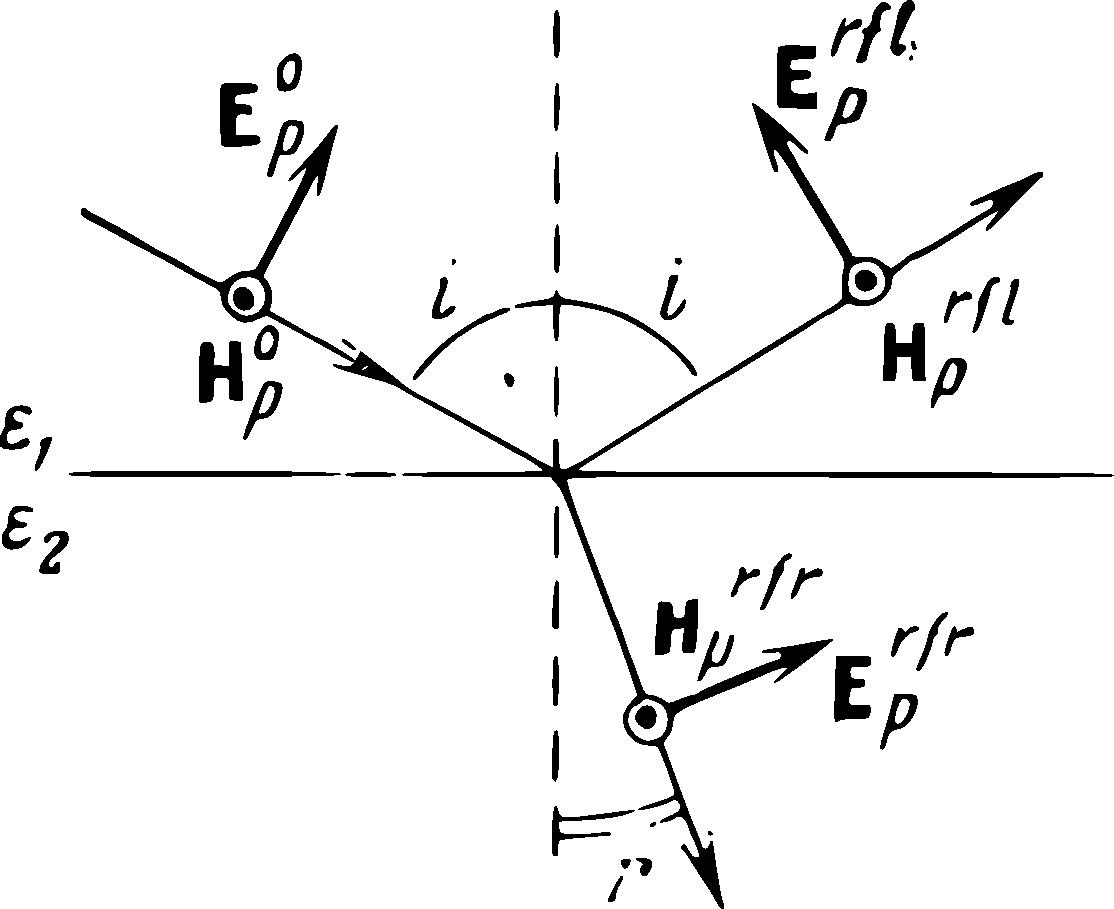
\includegraphics[width=\textwidth]{figs/ch-31/fig-31-06.pdf}
\sidecaption{$P$-waves reflected and refracted from interface of the media.\zhcap{$P$ 波在介质分界面上的反射与折射。}\label{fig-31-06}}
\end{marginfigure}
\begin{enumerate}[label=(\alph*)]
\item The reflected and refracted waves are also monochromatic
waves of the same frequency as the incident one.
\zhpar{反射波与折射波也是与入射波频率相同的单色波。}
\item The \redem{law of reflection} states that the reflected ray lies in the plane of incidence, and the angle of reflection is equal to the angle of incidence $(i' = i)$.
\zhpar{\redem{反射定律}：反射线位于入射面内，且反射角等于入射角（$i' = i$）。}
\item The \redem{law of refraction} states that the refracted ray lies in the plane of incidence and that the refractive angle is related to the angle of incidence by \redem{Snell's law}:
\zhpar{\redem{折射定律}：折射线位于入射面内，且折射角与入射角之间的关系由\redem{斯涅耳定律}给出：}
\begin{equation*}%
\frac{\sin i}{\sin r} = \frac{n_{2}}{n_{1}} = n_{21}.
\end{equation*}
\end{enumerate}


 
\subsection{}\label{31.5.4} Making use of the boundary conditions \ssect{31.5.3} the relations can be found between the phases, amplitudes and intensities of incident, reflected and refracted monochromatic waves.
\zhpar{利用边界条件\ssect{31.5.3}，可以求出入射波、反射波与折射波的相位、振幅与强度之间的关系。}


It is sufficient for this purpose, according to \ssect{31.1.8}, to know the above-indicated relations for linearly polarized waves of two types: \redem{p-waves}, whose vector $\vb{E} = \vb{E}_{p}$ lies in the plane of incidence and whose vector $\vb{H} = \vb{H}_{p}$ is perpendicular to this plane (\figr{fig-31-06}), and \redem{s-waves}, whose vector $\vb{E} = \vb{E}_{s}$ is perpendicular to the plane of incidence and whose vector $\vb{H} = \vb{H}_{s}$ lies in this plane (\figr{fig-31-07}).
\zhpar{为此，根据\ssect{31.1.8}，只需知道下述两类线偏振波的上述关系即可：\redem{$p$ 波}，其矢量 $\vb{E} = \vb{E}_{p}$ 位于入射面内，而其矢量 $\vb{H} = \vb{H}_{p}$ 垂直于该平面（见\figr{fig-31-06}）；以及\redem{$s$ 波}，其矢量 $\vb{E} = \vb{E}_{s}$ 垂直于入射面，而其矢量 $\vb{H} = \vb{H}_{s}$ 位于该平面内（见\figr{fig-31-07}）。}
\begin{marginfigure}%[-1.5cm]
\centering
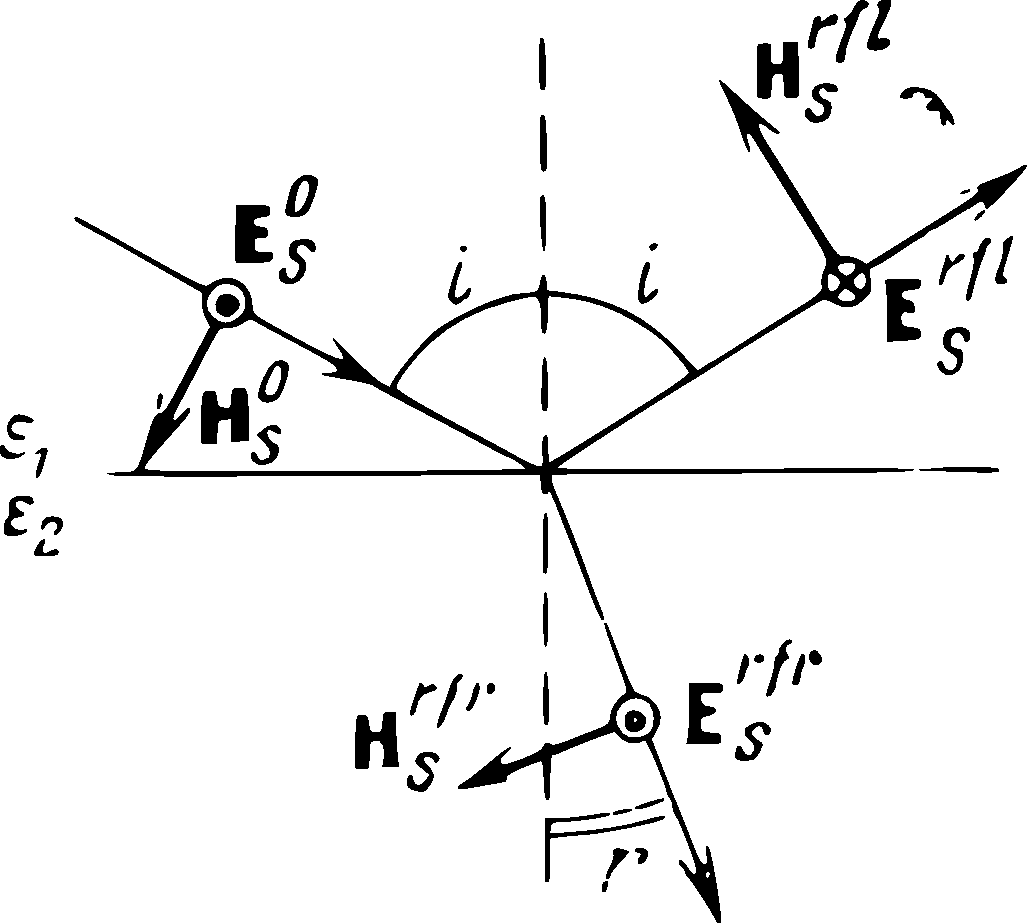
\includegraphics[width=\textwidth]{figs/ch-31/fig-31-07.pdf}
\sidecaption{$S$-waves reflected and refracted from interface of the media.\zhcap{$S$ 波在介质分界面上的反射与折射。}\label{fig-31-07}}
\end{marginfigure}
The relations between the amplitudes of oscillation of vector $\vb{E}$ in the incident $(A^{0})$, reflected $(A^{\text{rfl}})$ and refracted $(A^{\text{rfr}})$ waves in the cases of $p$- and $s$-waves are expressed by the \redem{Fresnel formulas}:
\zhpar{对于 $p$ 波与 $s$ 波，入射波 $(A^{0})$、反射波 $(A^{\text{rfl}})$ 与折射波 $(A^{\text{rfr}})$ 中矢量 $\vb{E}$ 振动振幅之间的关系，由\redem{菲涅耳公式}给出：}
\begin{align*}%
A^{\text{rfl}}_{p} & = - A_{p}^{0} \frac{\tan (i -r)}{\tan (i +r)}, & \quad A^{\text{rfr}}_{p} & = A_{p}^{0} \frac{2 \cos i \sin r}{\sin (i + r) \cos (i -r)},\\
A^{\text{rfl}}_{s} & = - A_{s}^{0} \frac{\sin (i -r)}{\sin (i +r)}, & \quad A^{\text{rfr}}_{s} & = A_{s}^{0} \frac{2 \cos i \sin r}{\sin (i + r)}.
\end{align*}
In particular, with normal incidence of waves on the interface
between media ($i = r = 0$),
\zhpar{特别地，当波垂直入射到两种介质的分界面上（$i = r = 0$）时，}
\begin{align*}%
A^{\text{rfl}}_{p} & = - A_{p}^{0} \frac{n_{21} -1 }{n_{21} + 1}, & \quad A^{\text{rfr}}_{p} & = A_{p}^{0} \frac{2 }{n_{21}+1},\\
A^{\text{rfl}}_{s} & = - A_{s}^{0} \frac{n_{21} -1}{n_{21} +1}, & \quad A^{\text{rfr}}_{s} & = A_{s}^{0} \frac{2}{n_{21}+1}.
\end{align*}
In the Fresnel formulas $A_{p}^{0}$ and $A_{s}^{0}$ are positive quantities, whereas $A_{p}^{\text{rfr}}$ and $A_{s}^{\text{rfr}}$ are also positive for any possible angles of incidence and refractive angles. This indicates that the refracted and incident waves are in phase. Quantities $A_{p}^{\text{rfl}}$ and $A_{s}^{\text{rfl}}$ can be either negative or positive. In the first case, illustrated in \figr{fig-31-06} and \figr{fig-31-07}, the phase of oscillation of vector $\vb{E}$ is changed by $\pi$ upon reflection (the phase of oscillation of vector $\vb{H}$ does not change). In the second case, the phase of oscillation of vector $\vb{E}$ remains unchanged (and, accordingly, the phase of oscillation of vector $\vb{H}$ changes by $\pi$).
\zhpar{在菲涅耳公式中，$A_{p}^{0}$ 与 $A_{s}^{0}$ 为正量，而 $A_{p}^{\text{rfr}}$ 与 $A_{s}^{\text{rfr}}$ 对于任何可能的入射角与折射角也都为正，这表明折射波与入射波同相。量 $A_{p}^{\text{rfl}}$ 与 $A_{s}^{\text{rfl}}$ 可以为负，也可以为正。在第一种情况下（如\figr{fig-31-06}与\figr{fig-31-07}所示），反射时矢量 $\vb{E}$ 的振动相位改变 $\pi$（矢量 $\vb{H}$ 的振动相位不变）。在第二种情况下，矢量 $\vb{E}$ 的振动相位保持不变（相应地，矢量 $\vb{H}$ 的振动相位改变 $\pi$）。}



\subsection{}\label{31.5.5} The values of the phase difference in the oscillation of vector $\vb{E}$ upon the reflection of $p-$ and $s-$type electromagnetic waves are listed in \tabl{tab-31-03}, in accordance with the conditions (i.e. depending on the angle of incidence $i$ and the relative refractive index $n_{21}$ of the media).
\zhpar{矢量 $\vb{E}$ 在 $p$ 型与 $s$ 型电磁波反射时的振动相位差，随条件（即入射角 $i$ 与两种介质的相对折射率 $n_{21}$）的不同而取值，列于\tabl{tab-31-03}中。}

The angle of incidence $i_{\text{Br}}$. at which the reflected and refracted rays are perpendicular to each other is called \redem{Brewster's angle}.
\zhpar{使反射线与折射线相互垂直的入射角 $i_{\text{Br}}$ 称为\redem{布儒斯特角}。}

When $i = i_{\text{Br}}$, then $i + r = \pi/2$ and it follows from the law  of wave refraction \ssect{31.5.3} that tan iBr = w21. It is evident from the Fresnel formulas \ssect{31.5.4} that at $i = i_{\text{Br}}$ the amplitude $A_{p}^{\text{rfl}} = 0$, i.e. the $p$-wave is not reflected from the interface between the media, but completely passes from medium $\mathit{1}$ into medium $\mathit{2}$.
\zhpar{当 $i = i_{\text{Br}}$ 时，$i + r = \pi/2$，由折射定律\ssect{31.5.3}可得 $\tan i_{\text{Br}} = w21$。由菲涅耳公式\ssect{31.5.4}可知，当 $i = i_{\text{Br}}$ 时振幅 $A_{p}^{\text{rfl}} = 0$，即 $p$ 波不在分界面上发生反射，而是全部从介质 $\mathit{1}$ 进入介质 $\mathit{2}$。}

\begin{table}[h!]
\centering
\begin{tabular}{@{\vspace{5pt}}p{1.75cm}p{1.25cm}p{1.25cm}p{1.25cm}p{1.25cm}@{}}
\toprule
\textbf{Condition} & \multicolumn{2}{c}{$i+r < \pi/2$} & \multicolumn{2}{c}{$i+r > \pi/2$ } \\
 & \multicolumn{2}{c}{ $(i < i_{\text{Br}}$)} & \multicolumn{2}{c}{ $(i > i_{\text{Br}}$)} \\
\midrule
\textbf{Wave Type} & $n_{21}> 1$ \newline $(i > r)$& $n_{21}< 1$ \newline $(i < r)$ & $n_{21}> 1$ \newline $(i > r)$ & $n_{21}< 1$ \newline $(i < r)$ \\
\midrule
$p$-wave & $\pi$ & 0 & 0 & $\pi$ \\
$s$-wave & $\pi$ & 0 & $\pi$ & 0 \\
\bottomrule
\end{tabular}
\sidecaption{The values of the phase difference in the oscillation of vector $\vb{E}$ upon the reflection of $p-$ and $s-$type electromagnetic waves.\zhcap{电磁波 $p-$ 型与 $s-$ 型波反射时，矢量 $\vb{E}$ 振动相位差的取值。}\label{tab-31-03}}

\end{table}


\subsection{}\label{31.5.6} The \redem{coefficient of reflection} (or \redem{reflection coefficient}) $R$ of an electromagnetic wave from the interface of two media is the ratio of the intensities \ssect{31.2.4} of the reflected and incident waves:
\zhpar{电磁波在两种介质分界面上的\redem{反射系数}（或称\redem{反射率}） $R$ 等于反射波与入射波的强度之比：}
\begin{equation*}%
R = \frac{I^{\text{rfl}}}{I_{0}} = \left( \frac{A^{\text{rfl}}}{A^{0}}\right)^{2}.
\end{equation*}
The reflection coefficients of the $p$- and $s$-waves are equal to
\zhpar{$p$ 波与 $s$ 波的反射系数分别为}
\begin{equation*}%
R_{p} = \frac{\tan^{2}(i -r)}{\tan^{2}(i +r)}, \quad R_{s} = \frac{\sin^{2}(i -r)}{\sin^{2}(i +r)}.
\end{equation*}
In particular, with normal incidence of waves on the interface
between two media $(i = r = 0)$
\zhpar{特别地，当波垂直入射到两种介质的分界面上（$i = r = 0$）时，}
\begin{equation*}%
R_{p} = R_{s} = \left( \frac{n_{21} -1 }{n_{21} + 1} \right)^{2}.
\end{equation*}
When the incident wave is arbitrarily polarized, the reflection
coefficient is
\zhpar{当入射波为任意偏振时，反射系数为}
\begin{equation*}%
R = \frac{I_{p}^{\text{rfl}} + I_{s}^{\text{rfl}}}{I_{p}^{0} + I_{s}^{0}} = \frac{R_{p} I_{p}^{0} + R_{s} I_{s}^{0}}{I_{p}^{0} + I_{s}^{0}}
\end{equation*}
where $I_{p}^{0}$ and $I_{s}^{0}$ are the intensities of the $p$- and $s$-components of the incident wave whose intensity is $I^{0} = I_{p}^{0} + I_{s}^{0}$.
\zhpar{式中 $I_{p}^{0}$ 与 $I_{s}^{0}$ 分别为入射波的 $p$ 分量与 $s$ 分量的强度，入射波的强度为 $I^{0} = I_{p}^{0} + I_{s}^{0}$。}

\subsection{}\label{31.5.7} The \redem{transmission factor}, or \redem{transmittance}, $T$ is the ratio of the intensity of the transmitted (refracted) wave to that of the incident wave. Thus
\zhpar{\redem{透射系数}（或称\redem{透射比}） $T$ 是透射（折射）波强度与入射波强度之比，即}
\begin{equation*}
T = \frac{I^{\text{rfr}}}{I_{0}} = \sqrt{\frac{\varepsilon_{r2}}{\varepsilon_{r1}}} \left(\frac{A^{\text{rfr}}}{A_{0}}\right)^{2} = n_{21} \left(\frac{A^{\text{rfr}}}{A_{0}}\right)^{2}.
\end{equation*}
The transmission factors for the $p$- and $s$-waves are
\zhpar{$p$ 波与 $s$ 波的透射系数分别为}
\begin{equation*}%
T_{p} = \frac{4 \cos^{2} i \sin i \sin r}{\sin^{2} (i + r) \cos^{2} (i -r)} \quad T_{s} = \frac{4 \cos^{2} i \sin i \sin r}{\sin^{2} (i + r)}.
\end{equation*}
In particular, upon normal incidence of waves on the interface
between media $(i = r = 0)$,
\zhpar{特别地，当波垂直入射到两种介质的分界面上（$i = r = 0$）时，}
\begin{equation*}%
T_{p} = T_{s} = \frac{4 n_{21}}{(n_{21} + 1)^{2}}.
\end{equation*}

\subsection{}\label{31.5.8} When $n_{21} =  (n_{2}/n_{1} ) < 1$ the refractive anprle is greater than the angle of incidence: 
\zhpar{当 $n_{21} =  (n_{2}/n_{1} ) < 1$ 时，折射角大于入射角：}
\begin{equation*}%
\sin r = \frac{\sin i}{n_{21}} \qand r > i. 
\end{equation*}
The angle of incidence at which the refractive angle becomes equal to $\pi/2$ is called the \redem{critical angle} $i_{cr}$. Angle $i_{cr} = \arcsin n_{21}$. When $i \geqslant i_{cr}$, the intensities of the reflected and incident waves are the same, i.e. the wave is completely reflected from the interface between the media $(R = 1)$. This phenomenon is called \redem{total internal reflection}.
\zhpar{使折射角等于 $\pi/2$ 的入射角称为\redem{临界角} $i_{cr}$，且 $i_{cr} = \arcsin n_{21}$。当 $i \geqslant i_{cr}$ 时，反射波与入射波的强度相同，即波在两种介质的分界面上被完全反射（$R = 1$）。这一现象称为\redem{全内反射}。}

\section{Doppler Effect}
\label{sec-31.6} 
\zhtitle{多普勒效应}




\subsection{}\label{31.6.1} Upon motion of the source and detector of electromagnetic waves toward each other the Doppler effect is observed \ssect{30.6.1}. The laws governing this phenomenon for electromagnetic waves can he established on the basis of the special theory of relativity.
\zhpar{当电磁波的源与探测器相互接近运动时，观察到多普勒效应\ssect{30.6.1}。这些电磁波的规律可根据狭义相对论来建立。}
\begin{marginfigure}%[-1.5cm]
\centering
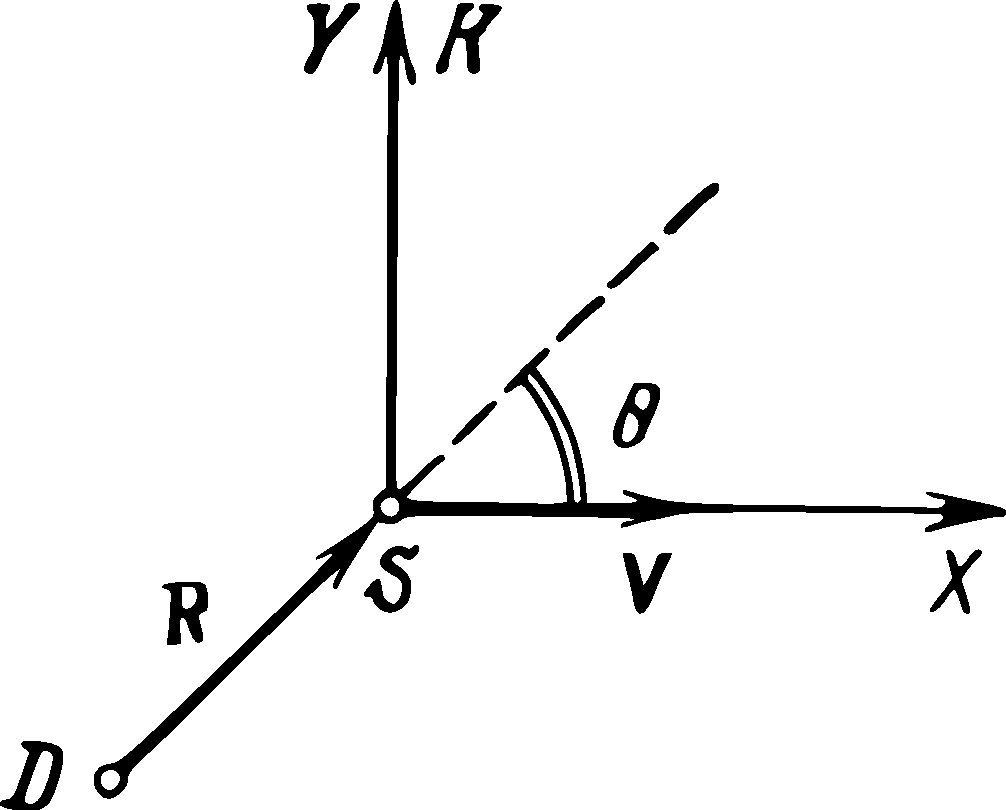
\includegraphics[width=0.8\textwidth]{figs/ch-31/fig-31-08.pdf}
\sidecaption{Source $S$ moving with velocity $\vb{V}$ in frame $K$.\zhcap{光源 $S$ 在参考系 $K$ 中以速度 $\vb{V}$ 运动。}\label{fig-31-08}}
\end{marginfigure}
Assume the detector $D$ to be stationary with respect to an inertial frame of reference $K$, and that the source $S$ travels with respect to $K$ along the positive direction of axis $OX$ at the velocity $\vb{V}$ (\figr{fig-31-08}). Source $S$ is stationary in frame of reference $K'$ and is located at its origin of coordinates. The axes of coordinate systems $K$ and $K'$ are parallel pairwise (axis $O'X'$ coincides with axis $OX$). Illustrated in \figr{fig-31-08} is the position of source $S$ at the instant of time $t = t' = 0$. 
\zhpar{设探测器 $D$ 相对于惯性参考系 $K$ 静止，光源 $S$ 相对于 $K$ 沿 $OX$ 轴正方向以速度 $\vb{V}$ 运动（见\figr{fig-31-08}）。光源 $S$ 在参考系 $K'$ 中静止，并位于其坐标原点。两参考系 $K$ 与 $K'$ 的坐标轴两两平行（轴 $O'X'$ 与轴 $OX$ 重合）。如\figr{fig-31-08}所示，为光源 $S$ 在时刻 $t = t' = 0$ 时的位置。}


According to Einstein's relativity principle \ssect{5.1.2}, the equation of a spherical monochromatic wave \ssect{30.2.8}, sent by the source at this instant of time in the direction of the detector $D$, is of identical form in frames of reference $K$ and $K'$:
\zhpar{根据爱因斯坦相对性原理\ssect{5.1.2}，光源在此时刻沿探测器 $D$ 方向发出的球面单色波方程\ssect{30.2.8}，在参考系 $K$ 与 $K'$ 中具有相同的形式：}
\begin{align*}%
\tilde{s} = \frac{a_{0}}{r} \exp i( \omega t + kx \cos \theta + ky \sin \theta + \delta) \tag{a} \qand \\
\tilde{s'} = \frac{a_{0}'}{r} \exp i( \omega' t' + k'x' \cos \theta' + k'y' \sin \theta' + \delta').\tag{b}
\end{align*}
Here $\omega' = \omega_{0}$ and $\omega$ are the angular frequencies of vibration of the source and detector, $k = \omega/c$ and $k' = \omega'/c$ are the wavenumbers (it is assumed that the wave propagates in vacuum), and $\theta$ and $\theta'$ are the angles between the directions of observation and of velocity $\vb{V}$ ($OX$ axis), measured in the frames
of reference of the detector $(K)$ and for the source $(K')$.
\zhpar{此处 $\omega' = \omega_{0}$ 与 $\omega$ 分别为光源与探测器的振动角频率，$k = \omega/c$ 与 $k' = \omega'/c$ 为波数（假设波在真空中传播），$\theta$ 与 $\theta'$ 分别为观测方向与速度 $\vb{V}$（$OX$ 轴）之间的夹角，分别在探测器参考系 $(K)$ 与光源参考系 $(K')$ 中测量。}

Expression (b) should be obtained from expression (a) by replacing the variables $x$, $y$ and $t$ by $x'$, $y'$ and $t'$ in accordance with Lorentz's transformations \ssect{5.3.2}:
\zhpar{式（b）应由式（a）按洛伦兹变换\ssect{5.3.2}，将变量 $x$、$y$ 与 $t$ 替换为 $x'$、$y'$ 与 $t'$ 而得到：}
\begin{align*}
\omega' t' & + k'x' \cos \theta' + k'y' \sin \theta' + \delta' \\
& \equiv \omega \left( \frac{t' + Vx'/c^{2}}{\sqrt{1 - (V/c)^{2}}} \right) 
+ k \left( \frac{x' + Vt'}{\sqrt{1 - (V/c)^{2}}} \right) \cos \theta 
+ k y' \sin \theta + \delta.
\end{align*}
Consequently,
\zhpar{由此可得：}
\begin{align*}
\omega' & = \frac{\omega}{\sqrt{1 - (V/c)^{2}}} \left( 1 + \frac{V}{c} \cos \theta \right), \\
k' \cos \theta' & = \frac{k}{\sqrt{1 - (V/c)^{2}}} \left( \cos \theta + \frac{V}{c} \right), \\
k' \sin \theta' & = k \sin \theta \qand \delta' = \delta.
\end{align*}
Hence, the relations describing the Doppler effect for electromagnetic waves in vacuum are of the form:
\zhpar{因此，真空中电磁波多普勒效应的关系式为：}
\begin{align*}
\omega & = \frac{\omega_{0} \sqrt{1 - (V/c)^{2}}}{1 + \frac{V}{c} \cos \theta} \qand \\
\nu & = \frac{\nu_{0} \sqrt{1 - (V/c)^{2}}}{1 + \frac{V}{c} \cos \theta}.
\end{align*}

\subsection{}\label{31.6.2} At low velocities of the wave source with respect to the detector $(V \ll c)$, the relativistic formula for the Doppler effect \ssect{31.6.1} coincides with the classical formula \ssect{30.6.3}:
\zhpar{当波源相对于探测器的速度很小（$V \ll c$）时，多普勒效应的相对论公式\ssect{31.6.1}与经典公式\ssect{30.6.3}一致：}
\begin{equation*}%
\nu \approx \nu_{0} \left( 1 - \frac{V}{c} \cos \theta \right).
\end{equation*}
When the source travels with respect to the detector along the
straight line that joins them (\theta = 0 or $\pi$ ), the \redem{longitudinal Doppler effect} is observed. If the source and detector approach each other $(\theta = \pi)$:
\zhpar{当光源相对于探测器沿连接二者的直线运动（$\theta = 0$ 或 $\pi$）时，观察到\redem{纵向多普勒效应}。若光源与探测器相互接近（$\theta = \pi$），则}
\begin{equation*}%
\nu = \nu_{0} \sqrt{\frac{1 + V/c}{1 - V/c}} > \nu_{0},
\end{equation*}
whereas if they travel away from each other $(\theta = 0)$,
\zhpar{而若二者相互远离（$\theta = 0$），则}
\begin{equation*}%
\nu = \nu_{0} \sqrt{\frac{1 + V/c}{1 - V/c}} < \nu_{0}.
\end{equation*}

\subsection{}\label{31.6.3} Following from relativistic theory of the Doppler effect \ssect{31.6.1} is the existence of the \redem{transverse Doppler effect}. It is observed when $0 = \pi/2$ and $\theta = 3\pi/2$, i.e. when the source
travels perpendicular to the line of observation. Thus
\zhpar{由电磁波多普勒效应的相对论理论还可推知\redem{横向多普勒效应}的存在。它出现在 $0 = \pi/2$ 与 $\theta = 3\pi/2$ 时，即光源沿垂直于观测方向运动时。于是有}
\begin{equation*}%
\nu = \nu_{0} \sqrt{1 - (V/c)^{2}}.
\end{equation*}
The transverse Doppler effect is substantially weaker than the
longitudinal effect (due to the smallness of $V/c$). This effect is due to the different passage of time in the frames of reference in which the detector and source of waves are fixed. Therefore, the experimental detection of the transverse Doppler effect was one of the most vital experimental proofs of the special theory of relativity.
\zhpar{横向多普勒效应比纵向效应弱得多（因为 $V/c$ 很小）。该效应源于探测器与波源所在参考系中时间流逝的不同。因此，横向多普勒效应的实验观测是狭义相对论最重要的实验证据之一。}

\subsection{}\label{31.6.4} The Doppler effect, associated with the thermal motion of the gas atoms that radiate light, leads to Doppler \redem{broadening of spectral lines}. The range of frequencies of light recorded by the detector extends from $\nu_{0} - \Delta \nu_{D}/2$ to $\nu_{0} + \Delta \nu_{D}/2$, where $\nu_{0}$ is the frequency of monochromatic radiation of a stationary atom. The amount of Doppler broadening $\Delta \nu_{D} \propto \sqrt{T/m}$, where $T$ is the absolute temperature and $m$ is the mass of the atom.
\zhpar{与发光气体原子热运动相关的多普勒效应，导致谱线的\redem{多普勒加宽}。探测器接收到的光频率范围从 $\nu_{0} - \Delta \nu_{D}/2$ 延伸到 $\nu_{0} + \Delta \nu_{D}/2$，其中 $\nu_{0}$ 为静止原子单色辐射的频率。多普勒加宽量 $\Delta \nu_{D} \propto \sqrt{T/m}$，其中 $T$ 为绝对温度，$m$ 为原子的质量。}